\documentclass[9pt]{beamer}
% ****************
% ***** INFO *****
% ****************
\usepackage[english]{babel}
\title[University of Calabria]{Magma intrusion in the crust: implications to the crustal dynamics.\\}
\subtitle{Supervisors: Prof. Mario La Rocca,\\\quad\quad\quad\quad  Prof.ssa Eleonora Rivalta,\\\quad\quad\quad\quad Dott. Francesco Maccaferri.}
\author[Name Surname]{ Francesco De Rose. \textbf{ID}: 256865}
\institute[]{University of Calabria, Physics department, Rende (CS). \\
National Institute of Geophysics and Volcanology (INGV), Naples Section - Vesuvius Observatory Napoli, Italy. \\ Department of Physics, Section of Geophysics, University of Bologna, V.le B. Pichat 8, Bologna , Italy.}
\newcommand{\currentyear}{\the\year} % \currentyear
\newcommand{\nextyear}{\the\numexpr\year+1\relax} % \nextyear
\date{\currentyear/\nextyear} % or \today
\setbeamertemplate{frametitle}[default][center]

% *******************
% ***** PROJECT *****
% *******************
\definecolor{main}{HTML}{0000FF}
\setbeamercolor{structure}{fg=main}

% *****************
% ***** THEME *****
% *****************
\usepackage{wrapfig}
\usetheme{Luebeck}
\usepackage{helvet}
\renewcommand{\familydefault}{\sfdefault}
\setbeamertemplate{frametitle continuation}{\gdef\beamer@frametitle{}}
\setbeamertemplate{footline}[frame number]

% *****************
% ***** CODE *****
% *****************
\newcommand\Fontsm{\fontsize{4}{5}\selectfont}
\newcommand\Fontvi{\fontsize{6}{7.2}\selectfont}
\newcommand\Fonttab{\fontsize{12}{7.2}\selectfont}
\usepackage{listings}
\lstdefinestyle{java}{
    backgroundcolor=\color{white},
    basicstyle=\ttfamily\scriptsize,
    breaklines=true,
    commentstyle=\color{gray},
    keywordstyle=\color{blue},
    stringstyle=\color{magenta},
    identifierstyle=\color{black},
    numberstyle=\color{gray},
    language=Java
}
\lstdefinestyle{cpp}{
    backgroundcolor=\color{white},
    basicstyle=\ttfamily\scriptsize,
    breaklines=true,
    commentstyle=\color{gray},
    keywordstyle=\color{blue},
    stringstyle=\color{magenta},
    identifierstyle=\color{black},
    numberstyle=\color{gray},
    language=C++
}
\lstdefinestyle{py}{
    backgroundcolor=\color{white},
    basicstyle=\ttfamily\scriptsize,
    breaklines=true,
    commentstyle=\color{gray},
    keywordstyle=\color{blue},
    stringstyle=\color{magenta},
    language=Python
}
\lstdefinestyle{js}{
    backgroundcolor=\color{white},
    basicstyle=\ttfamily\scriptsize,
    breaklines=true,
    commentstyle=\color{gray},
    keywordstyle=\color{blue},
    stringstyle=\color{magenta},
    identifierstyle=\color{black},
    numberstyle=\color{gray},
    language=JavaScript,
    escapechar=@
}
\lstdefinestyle{sh}{
    basicstyle=\ttfamily\scriptsize,
    breaklines=true,
    commentstyle=\color{gray},
    keywordstyle=\color{blue},
    stringstyle=\color{magenta},
    identifierstyle=\color{black},
    numberstyle=\color{gray},
    language=bash
}

% **********************
% ***** ALGORITHMS *****
% **********************
\usepackage{algorithm}
\usepackage{algpseudocode}

% *****************
% ***** UTILS *****
% *****************
\usepackage{xcolor}
\usepackage{graphicx}
\graphicspath{./figs/}
\usepackage[makeroom]{cancel}
\newcommand\Ccancel[2][black]{\renewcommand\CancelColor{\color{#1}}\cancel{#2}}
% ********************
% ***** DOCUMENT *****
% ********************
\begin{document}

% **********************
% ***** TITLEPAGE ******
% **********************
\begin{frame}{}
\vspace{\fill}
  
\begin{wrapfigure}{r}{0.30\textwidth}
    \centering
    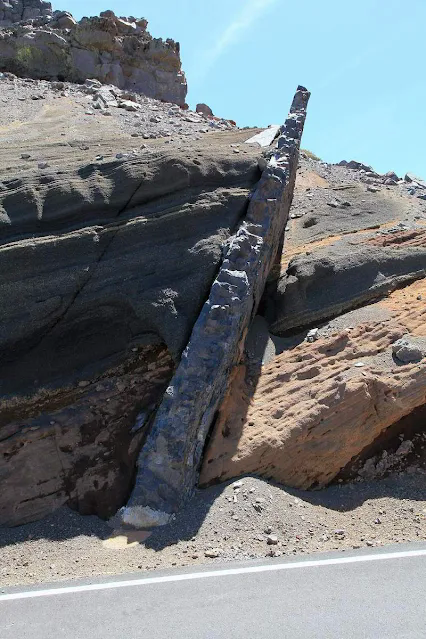
\includegraphics[height=0.45\textwidth]{/figs/copertina.png}
\end{wrapfigure}

\vspace{\fill}
\begin{figure}[h]
    \centering
    
\includegraphics[width=0.45\textwidth]{/figs/logof.jpg}
\end{figure}
\Large
\color{main}
\inserttitle

\medskip

\large
\color{black}
\insertsubtitle

\vspace{\fill}

\footnotesize
\insertinstitute

\vspace{\fill}

\textbf{Candidate:} \insertauthor 

\medskip

\textbf{Academic year:} 2024/2025

\begin{figure}[h]
    \centering
    
\includegraphics[width=0.10\textwidth]{/figs/unibo.png}
    
\includegraphics[width=0.10\textwidth]{/figs/ingv.png}
\end{figure}

\end{frame}

\begin{frame}[allowframebreaks]{\textbf{Introduction}}
\Fonttab
\begin{itemize}
\item This presentation focuses on the study of a new modeling scheme for the  \textbf{dykes shapes} evolution and propagation in time, using a Fortran90 code\footnote{ \url{https://zenodo.org/records/3957577}, \, \url{https://zenodo.org/records/7118734}}.
\item In the case studied a \textbf{2D BE} technique, depending on the variable opening $h_i \in [1,\cdots , N]$ has been implemented.
%\textit{Italic}
\item The modules \texttt{BELEMENT\_4FE-STRESS\_DYN-CRACK.f90} deals with the \textbf{magma parameters} depending on the user input and \texttt{COMP\_FIELD\_4FE-STRESS.f90} takes care of the stress components in the problem through the "\texttt{input\_field.dat}" while the \texttt{DISL2D.f90} and \texttt{EXTERNAL\_FIELD.f90} deals with the RHS routine.  
\end{itemize}
\begin{eqnarray}
\boxed{\rho \ddot{\bf u}  - \rho \bf{F} - \nabla \cdot \bf{\sigma} = \text{0}}
\end{eqnarray}
\end{frame}

\begin{frame}[allowframebreaks]{\textbf{Magma ascent mechanisms}}
\Fonttab
\begin{columns}[onlytextwidth,T]
      \column{\dimexpr\linewidth-40mm-5mm}
Rock mechanics is fundamental in the formation of igneous rocks, which are created during magma ascent. \\
The interaction between fluid dynamics, thermodynamics, and rock mechanics influences the propagation of magma, affecting crustal stresses and rheology \colorbox{yellow}{\cite{maccaferri2011}}. \\
This in turn makes possible the development of natural resources like ore deposits and petroleum reservoirs, as well as an impact on human life.
      \column{80mm}
    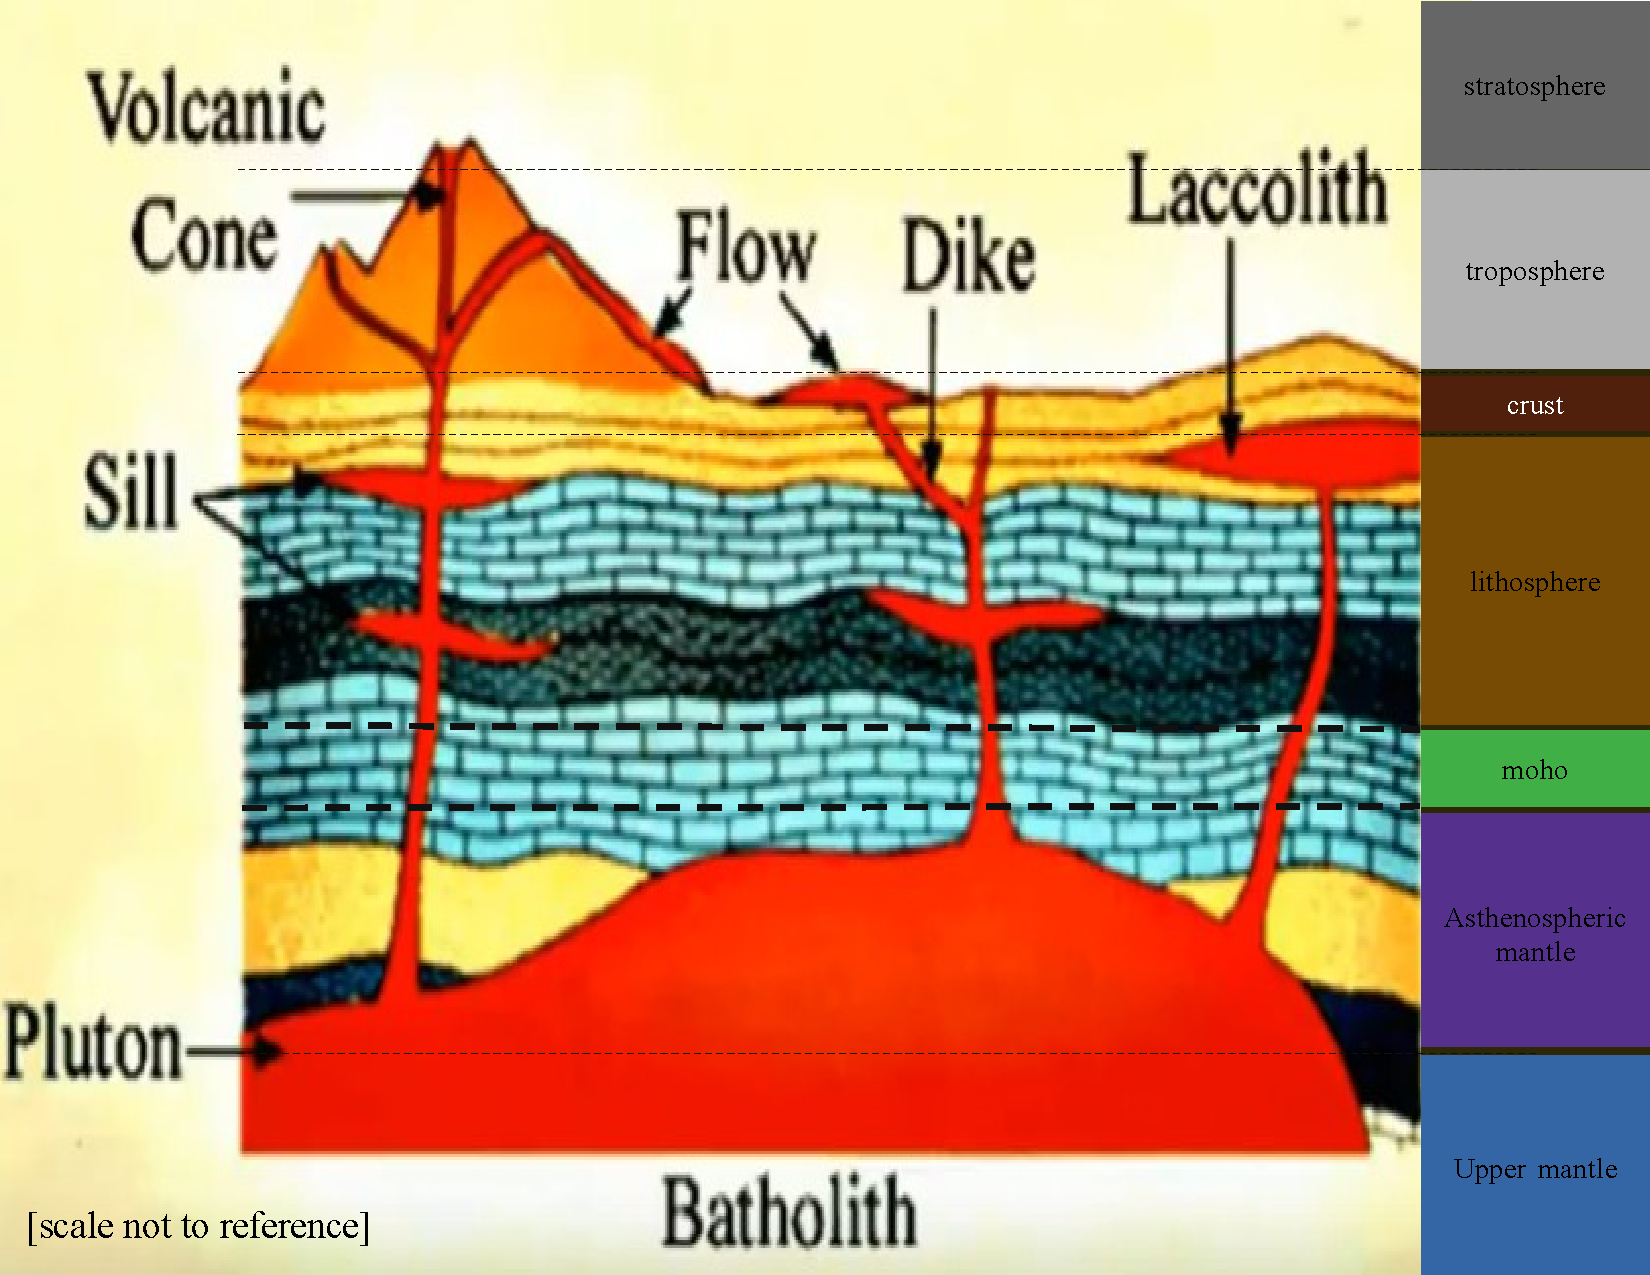
\includegraphics[width=0.6\textwidth]{/figs/dykes_scheme.pdf}
    \end{columns}
\end{frame}

\begin{frame}[allowframebreaks]{\textbf{Types of dykes}}
Dikes can \colorbox{yellow}{\cite{rivalta2015}}:
\begin{enumerate}
\item be segmented or straight, 
\item can deviate in orientation, can get arrested at layer discontinuities 
\item cut through heterogeneous or pre-existing fractures., deviate projection along the discontinuity, or cut through it unaffected by the discontinuity.\\
\end{enumerate}
Low-viscosity magmas may form intricate networks generated by mutually cross-cutting dikes.\\
Seismically-inferred velocities of dike propagation range from \underline{1 km/day} to a \underline{few km/hour}. 
    \Fontsm
    \begin{figure}
        \centering
    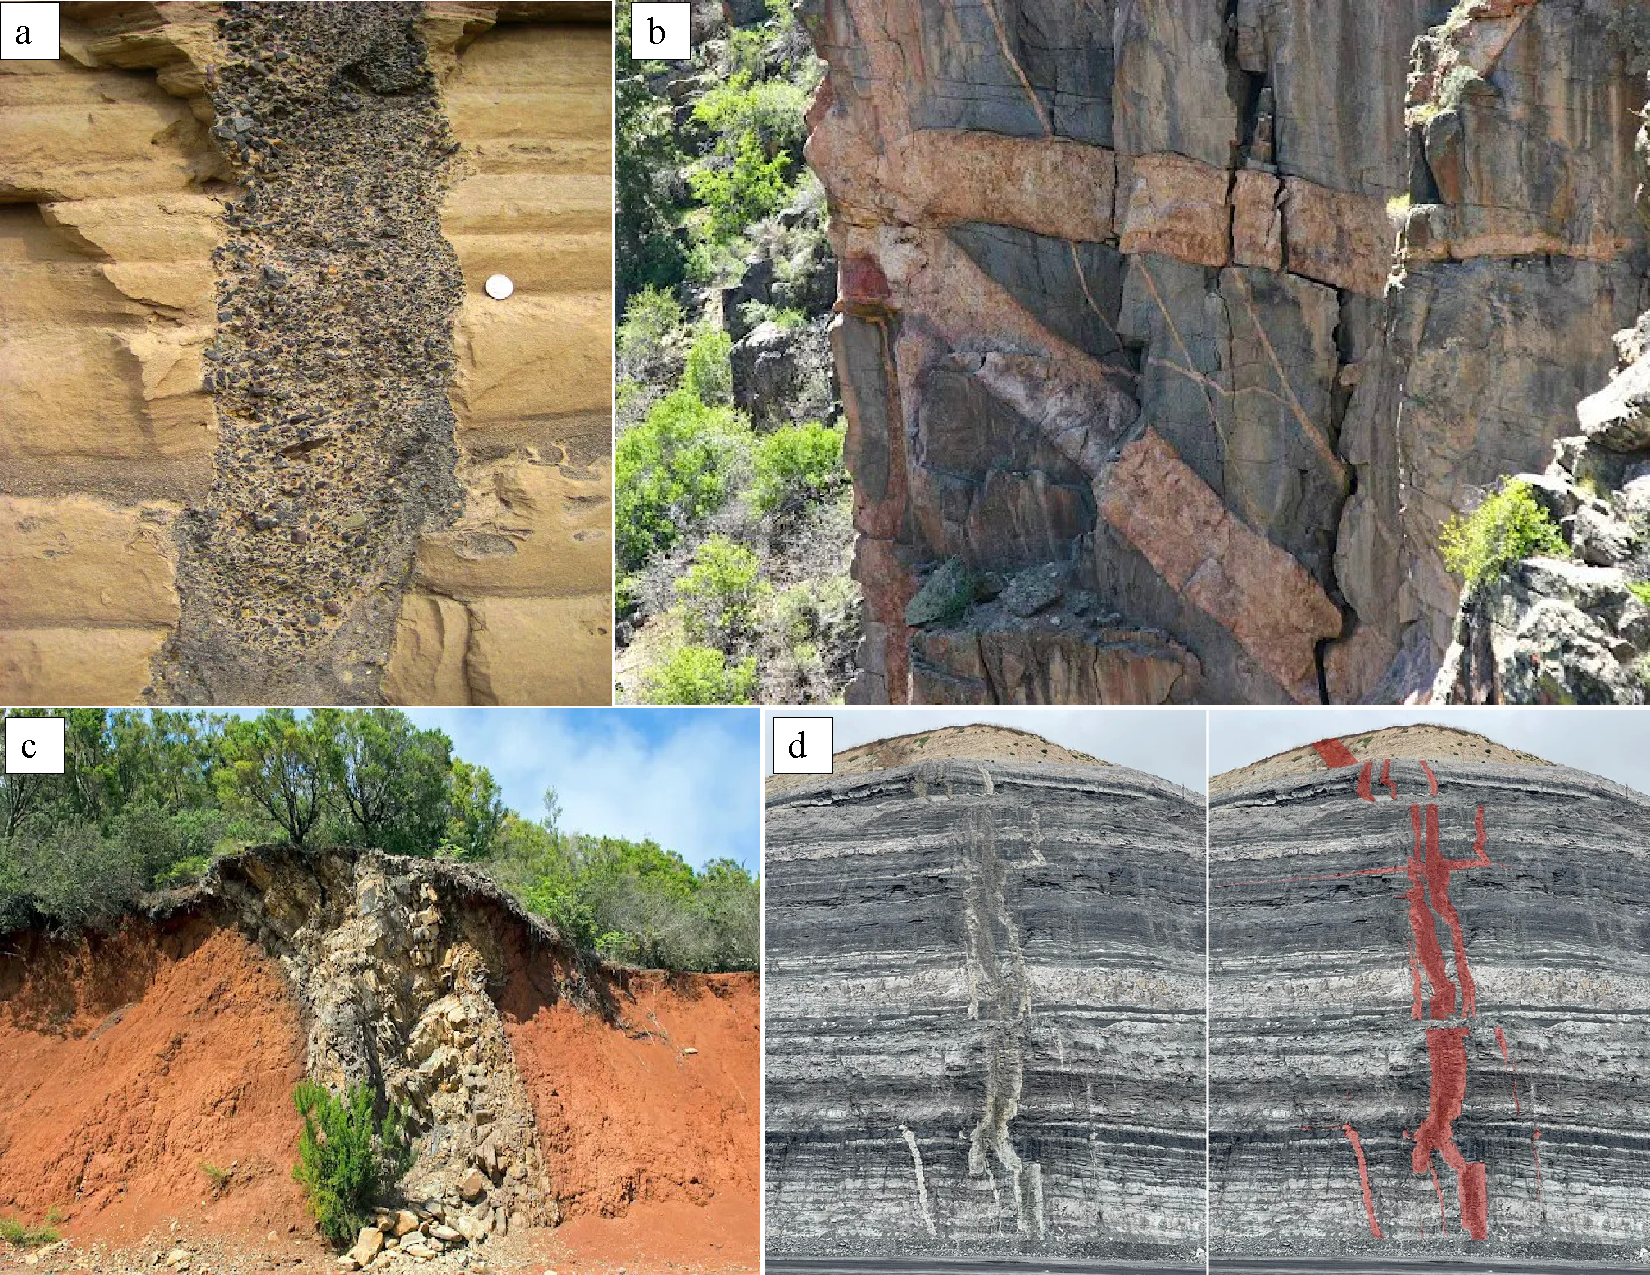
\includegraphics[width=0.60\textwidth]{/figs/dykes.pdf}
    \caption{(a) Clastic dike; (c) Volcanic dike. Mass of igneous rock intruded into older red iron rich sedimentary rock. 1km north of Garajonay summit, La Gomera; (b) Volcanic sill; (d) Complex dyke geometry of alternating layers of mudstone and sandstone, probably deposited in a deep somewhat anoxic basin, exposed by mining in the Hunter Valley, NSW.}
    \end{figure}
\end{frame}

\begin{frame}[allowframebreaks]{\textbf{Dykes evolution and movement}}
\Fontvi
The problem of elasticity involves determining the stresses and displacements of a body subjected to prescribed tractions and forces at its interior points. The figure below depicts two of the \underline{typical assumptions} one makes when trying to model the dyke evolution in space and time. \\
    \begin{figure}
        \centering
    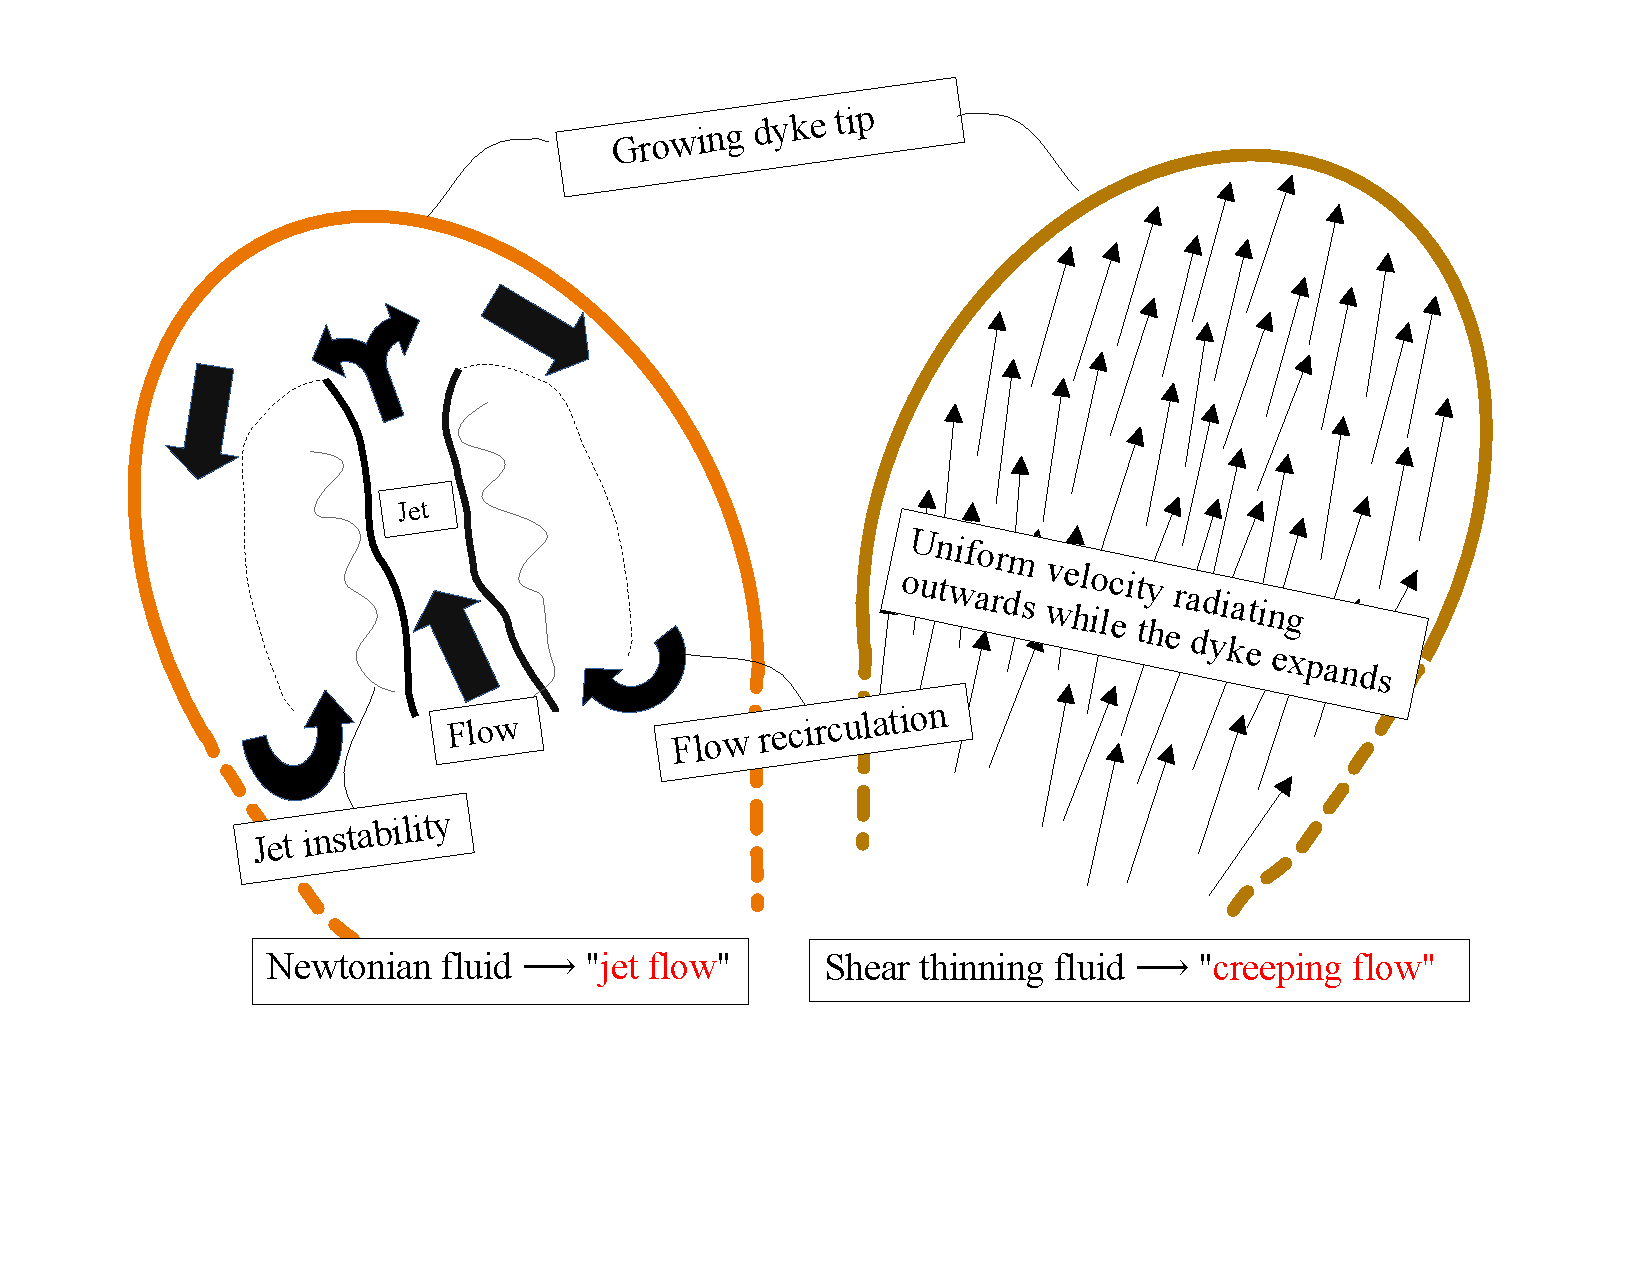
\includegraphics[width=0.64\textwidth]{/figs/flow_regimes.pdf}
    \end{figure}
    The aim is having a \underline{small magma viscosity} that will dissipate the energy in the small scales but not affect the larger scales, given the fluid flow assumption \colorbox{yellow}{\cite{peltier2007}}.
\end{frame}


\begin{frame}[allowframebreaks]{\textbf{Governing equations}}
\begin{enumerate}
\item Elasticity problem
\begin{eqnarray}
\boxed{ \Ccancel[red]{\rho \ddot{\bf u}}  - \rho \bf{F} - \nabla \cdot \bf{\sigma} = \text{0}} \,  \longrightarrow \, \boxed{(\lambda + \mu ) \nabla (\nabla \cdot \bf u)  + \mu \nabla^2 \bf{u} - \rho \bf{F} = 0}
\end{eqnarray}
\item Fluid description inside the crack fracture (\underline{Poiseuille flow} within piece-wise parallel fracture walls)
\begin{eqnarray}
-{\frac{1}{\eta}}{\frac{\partial P_{v i s c}}{\partial s}}={\frac{d^{2}u_s}{d r^{2}}}, \quad \frac{\partial(\rho_{m}(s,t)h(s,t))}{\partial t}=-\frac{\partial(\rho_{m}(s,t)f(s,t))}{\partial s}
\end{eqnarray}
\Fontvi
\item Energy conservation inside the volume
\begin{eqnarray}
{\frac{\partial W}{\partial t}}+{\frac{\partial G}{\partial t}}-{\frac{\partial}{\partial t}}(E_{f}\cdot d s+E_{\nu})=0 , \quad E_{f}=K_{c}^{2}\,{\frac{1-\nu}{2\mu}}. \colorbox{yellow}{\cite{dahm2000a}}
\end{eqnarray}
\item Incompressibility condition leads to
\begin{eqnarray}
f_{i}^{t o p}=-v\sum_{j=1}^{i}\left(h_{j}^{k}-\frac{V^{k}}{V^{k-1}}h_{j}^{k-1}\right) \xrightarrow{[...]}f_{i}=-\Gamma_{i}\cdot\frac{\left(h_{i}^{k-1}\right)^{3}}{12\eta} , \,  \Gamma_{i}=\frac{\partial P_{v i s c}(s,t)}{\partial s}\bigg|_{i}
\end{eqnarray}
\item Solving iteratively \colorbox{yellow}{\cite{furst2023}}
\begin{eqnarray}
\Delta P_{visc,i}=l\cdot\left(\sum_{m=1}^{i}\Gamma_{m}-\frac{1}{2}\Gamma_{i}\right) \, \text{with} \, i \in [1, .., N-1] \\ \Delta P_{N}^{v i s c}=\Delta P_{N-1}^{v i s c}+\frac{l}{2}\Gamma_{N}\,\text{and}\, f_{N}=\frac{1}{2}v h_{N}^{k}
\end{eqnarray}
\end{enumerate}
\centering
\end{frame}

\begin{frame}[allowframebreaks]{\textbf{Dyke propagation school of thoughts}}
\Fonttab
If one considers the numerical approaches to this problem:
\begin{enumerate}
\item \textbf{The Weertman school} uses static crack theory and quasi-static approaches, disregarding fluid motion. These models provide indirect information about crack propagation velocity and can be used \underline{when energy dissipated by viscous flow is negligible} \cite{Weertman1971}. 
\end{enumerate}
\begin{enumerate}
\item \textbf{The lubrication theory} school simplifies crack geometry and crustal stress but accounts for the \underline{interaction between elastic forces and viscous forces} due to fluid motion \cite{lecampion2018}.  
\end{enumerate}
These models can quantify changes in crack propagation velocity due to dynamic changes in the magma source or variations in crust and stress properties. \colorbox{yellow}{\cite{furst2023}} code is able to \underline{take some aspects from both approaches}.
\end{frame}

\begin{frame}{\textbf{Dyke propagation numerical modeling and its limits}}
\Fonttab
In the single layer case a stress-free regime has been defined while with a double layer case an horizontal strain case has been analyzed, where the user is more interested in the dike's propagation path and shape rather than the stress/displacement fields induced by it \colorbox{yellow}{\cite{maccaferri2011}}.
    \begin{alertblock}{Implementation Details}
        \begin{enumerate}
            \item The simulation domain is a $20 \times 20$ km square.
            \item The input stress grid is very coarse ($10$ km step).
            \item Stress and displacement fields from the dike will not be computed (\texttt{comp\_dyke\_stress-displ = .false.}).
            \item The output resolution for principal stress directions ($0.5$ km step) is finer than the input grid.
            \item The dike's shape is printed every $5$ km of vertical propagation, with its opening exaggerated by a factor of $0.100$ (a factor of $2.5$ is used in the final figures).
        \end{enumerate}
    \end{alertblock}
\end{frame}

\begin{frame}[allowframebreaks]{\textbf{Energy budget and problem initialization}}
\Fonttab
\begin{exampleblock}{Note}
Looking at the fig.\ref{fig:rheo}, there are main regimes one can look within the choice of rock parameters as well as crack shapes geometry \cite{pansino2022}. After validating the code with some trial runs it has been found it is very sensible to the velocity balancing the energy budget contributions. All runs have considered a single dyke even though one could define multiple structures in the appropriate input files. 
\end{exampleblock}
\begin{figure}[b]
    \centering
    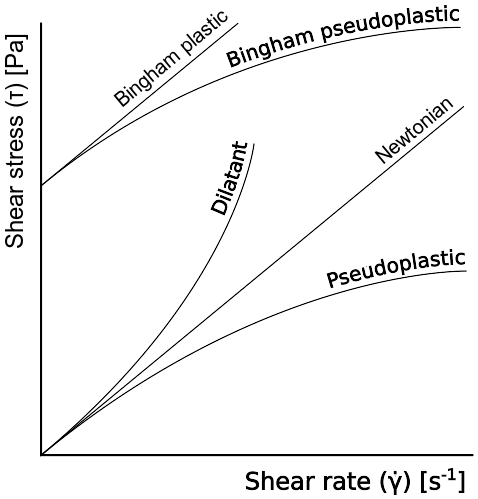
\includegraphics[height=0.3\textwidth]{/figs/rheologyfluids.png}
    \label{fig:rheo}
\end{figure}
\end{frame}

\begin{frame}[allowframebreaks]{\textbf{Velocity balancing energy budget subroutine}}
\begin{figure}[h]
    \centering
    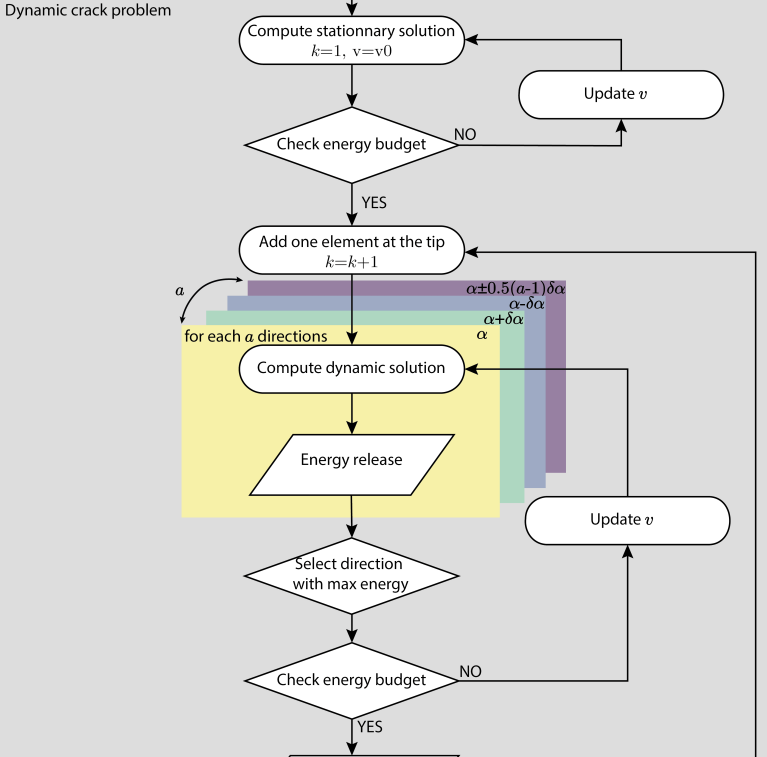
\includegraphics[width=0.4\textwidth]{/figs/dyn_crackprobl.png}
    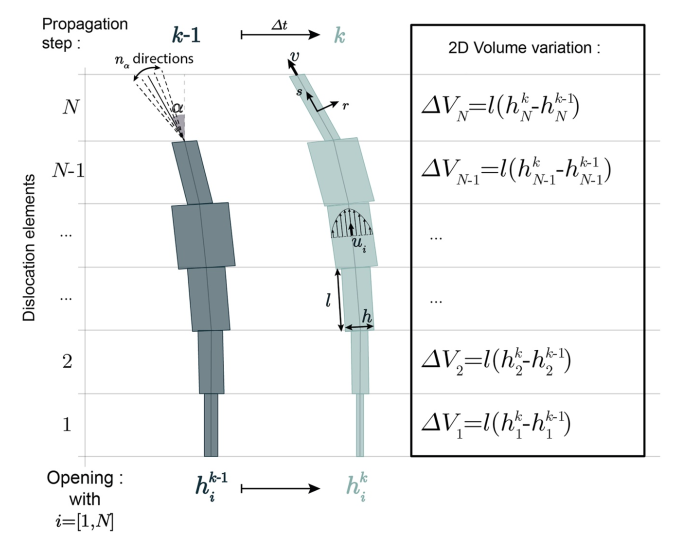
\includegraphics[width=0.4\textwidth]{/figs/be_scheme.png}
    \caption{Diagram representing main steps of the new numerical approach described in \colorbox{yellow}{\cite{furst2023}}. The numerical approach stops either when the crack tip has reached a prescribed depth (z = \texttt{zstop} ), or when the number of propagation steps has reached a prescribed value (k = \texttt{kiter}); see also \colorbox{yellow}{\cite{dahm2000a}\cite{dahm2000b}}. Various stress regimes have been set up in the simulations which have reached stable convergence.}
\end{figure}
\end{frame}

\begin{frame}[allowframebreaks]{\textbf{Simulations and results - what has been plotted}}
\Fonttab
\begin{enumerate}
\item \textbf{Dyke shape} Numerical crack shape as the iteration steps increase and overlayed one.
\item \textbf{Velocity} v(x,t) w.r.t. the Pousille fluid flux to show the different regimes, velocity w.r.t. dyke tip depth.
\item \textbf{Energy} variation over the iteration step along i, \underline{total number of time steps}.
\item \textbf{Pressure} For every case the overpressure and viscous pressure has been plotted.
\end{enumerate}
% ******* TABLES *********
\Fontsm
\begin{table}[h]
    \centering
    \begin{tabular}{|c|c|c|c|c|c|c|c|c|c|}
    \hline
        \textbf{SIM} & \textbf{$\mu$ [GPa]} & \textbf{$E_f$ [MPa·m]} & \textbf{$K_c$ [MPa$\sqrt{\text{m}}$]} & \textbf{$v_i$ [mm/s]} & \textbf{$\eta$ [Pa·s]} & \textbf{$A_0$ [km$^2$]} & \textbf{$\delta_0$ [°]} & \textbf{$\Delta \rho$ [dg/cm$^3$]} & \textbf{$\nu$} \\
    \hline
        A1 &20 &20 &1033 &5.33 &0.5 &0.009 & 0 &300 & 0.25 \\ \hline
        A2 &20 &14 &864  &1.5  &100 &0.009 & 0 &300 & 0.25 \\ \hline
        A3 : A3.6 &22 ~ &14 ~ & 906~ &1.5 ~ & [*]~ &0.009 ~ &0 ~ &300 ~ &0.25 ~ \\ \hline
        A4 &21 ~ &11 ~ &796 ~ &1.5 ~ & 100~ & 0.009~ &15 ~ &150 ~ &0.27 ~ \\ \hline
        A5 &24 &14~ &928 ~ &1.5 ~ &100 ~ &0.009~ &30~ &200&0.22 ~ \\ \hline
        A6 &18~ &12 ~ &749 ~ &1.5 ~ &100 ~ &0.009 ~ &45 ~ &250 ~ &0.23 ~ \\ \hline
        A7 &15~ &12~ &688 ~ &1.5 ~ &100 ~ &0.009 ~ &60 ~ &300 ~ & 0.24~ \\ \hline
        A8 &20~ &4.6~ &495 ~ &5.331 ~ &100 ~ &0.009 ~ &0 ~ &300 ~ &0.25 ~ \\ \hline
    \end{tabular}
    \caption{Rock and fluid coefficients and various quantities computed for runs in Set A. If possible, the dyke was initialized with inclination angle $\delta_0 \in [0^\circ,\,60^\circ]$. [*]=[100, 316, 400,425;250,500(in the last two values $E_f$ was raised to 16),750].}
\end{table}
%double layer values
\begin{table}[!ht]
    \centering
\begin{tabular}{|c|c|c|c|c|c|c|c|c|c|c|}
    \hline
    \textbf{SIM} & \textbf{$\Delta\mu$}[GPa] & \textbf{$\Delta E_f$} [MPa m] & \textbf{$\Delta K_c$ }[MPa$\sqrt{\text{m}}$] & \textbf{$v_i$} [mm/s] & \textbf{$\eta$ }[Pa·s] & \textbf{$A_0$} [km$^2$]  & \textbf{$\Delta \rho$ }[dg/cm$^3$] & \textbf{$\rho_f$ }[kg/dm$^3$] & \textbf{$\nu$} & \textbf{$K_f$} [GPa] \\
    \hline
    B1 &10 ~ &8 ~ &302 ~ &0.5 ~ &500 ~ &0.009 ~ &200 ~ &2.7 ~ &0.25 ~ &15 ~ \\ \hline
    B2 &12 ~ & 8~ &270 ~ &1.2 ~ &20 ~ &0.012  ~ & 300~ &2.6 ~ &0.25 ~ &10 ~ \\ \hline
    B3 & 5~ &8 ~ &270 ~ &1.2 ~ &20 ~ & 0.012 ~ &100 ~ &2.6 ~ &0.25 ~ &10 ~ \\ \hline
    B4 &15 ~ &8 ~ &299 ~ &1.9 ~ &20 ~ &0.009  ~ &500 ~ &2.7 ~ &0.23 ~ &18~ \\ \hline
    B5 &5 ~ &8 ~ &270 ~ & 4.0~ & 95~ &0.011  ~ &200 ~ &2.6 ~ &0.25 ~ &10~ \\ \hline
    B6 &17 ~ &8 ~ &302 ~ &1.0 ~ &10 ~ &0.009  ~ &200 ~ &2.6 ~ &0.25 ~ &12 ~ \\ \hline
    B7 &10 ~ &8 ~ &271 ~ &0.5 ~ & 25~ &0.009  ~ &350 ~ &2.6 ~ &0.25 ~ &15 ~ \\ \hline
    B8 &10 ~ &9 ~ &278 ~ &5.0 ~ &5.0 ~ &0.007 ~ &300 ~ &2.5 ~ &0.22 ~ &19 ~ \\ \hline
    B9 &10 ~ &8 ~ &270 ~ &0.8 ~ &100 ~ &0.009 ~ &0 ~ &2.7 ~ &0.25 ~ &20 ~ \\ \hline
\end{tabular}
    \caption{Rock and fluid coefficients and various quantities computed for runs in Set B. $A_0$ is the "critical length for propagation" according to Weertman theory. The dyke was initialized with a nonzero dip angle only in case B7 ($\delta_0=30^\circ$) in a no-stress regime while in case B8 an horizontal stress (compressional) configuration was selected, namely $\sigma_{xx}=5 \, MPa$ inside the numerical grid with 10 km stepsize. For more info see the the relative \texttt{input\_field.dat} for the case shown.}
\end{table}

\end{frame}
% ******* FIGURES ********
\begin{frame}{\textbf{Numerical velocity computation - case A1, A1-8}}
Below Figure \ref{fig:1}, show the numerical crack tip velocity w.r.t. the theoretical one (see \cite{turcotte1990}. $t^{\star}=A_0^2 g \Delta \rho t / \pi^2 (L/2)^3 \eta$ and $v_{th}=(A_0^2 \Delta \rho g/48 \eta t^2)^{1/3}$; also the velocity w.r.t. the viscosity has been plotted.
\begin{table}
    \centering
    \begin{tabular}{cc}
            \includegraphics[width=0.45\linewidth]{figs/fgs/1lay/case1/1l_veln_th_case1.pdf}
        \includegraphics[width=0.45\linewidth]{/figs/fgs/1lay/1lcrckvel.png}
    \end{tabular}
    \label{fig:1}
  \caption{If $\sigma_{xx}<0$, tensile stresses make it more easy for dykes to develop a vertical opening \colorbox{yellow}{\cite{furst2024}}, therefore, for the single case, the input density of the material surrounding the fluid rising has been defined accordingly. For the double layer, the density variation between the two layers was used.
The stress regimes for cases B1- B6,B9 has always been a generic basaltic dyke in an horizontal extensional regime, subject to a gradually increasing vertical stress and shear stress of 2 MPa in upper crust and 4 MPa in lower crust. Different regimes depending on the density contrast or the fluid viscosity or fracture opening have been modified in the subsequent runs.}
\end{table}
\end{frame}

\begin{frame}{\textbf{Energy variation throughout the runs - case A1,A3,A3.5,A4,A6,A8}}
\Fontvi
Figure \ref{fig:2} show the total energy, released by the dyke propagating in the direction, according to which the max energy release is reached (by subtracting the total energy, associated with the propagation in each direction, to the previous iteration energy value). Gradually decreasing the fracture toughness seems to decrease the time needed to reach the energy plateau, ex: A4, A6.
\begin{table}
    \centering
    \begin{tabular}{cc}
        \includegraphics[width=0.75\linewidth]{/figs/fgs/1lay/1l_enrgvar_case1.pdf}
    \end{tabular}
    \label{fig:2}
\end{table}
\end{frame}

\begin{frame}{\textbf{Pressure trend throughout the runs - case A5,A8}}
Below Figure \ref{fig:3}, show the overpressure estimate along the crack printed at each iteration step at dislocation element and viscous pressure drop at the same element number.
\begin{table}
    \centering
    \begin{tabular}{cc}
        \includegraphics[width=0.45\linewidth]{figs/fgs/1lay/case5/ovep_vscp_case5.pdf}
        \includegraphics[width=0.45\linewidth]{figs/fgs/1lay/case8/ovep_vscp_case8.pdf}
    \end{tabular}
    \label{fig:3}
  \caption{ On the left (A5) a sharp increase in overpressure is observed near the crack tip, likely reflecting stress concentration and the need to overcome fracture toughness at the front of the dyke. The interior ends maintain a lower, relatively uniform pressure. On the right (A8), overpressure shows a non-monotonic variation, peaking mid-crack before dropping toward the tip, which may suggest local impedance in magma flow or even variable stiffness along the fracture walls. Other cases were not particularly interesting since the overall increase$\backslash$decrease for overpressure$\backslash$viscous pressure was always seen.}
\end{table}
\end{frame}

\begin{frame}{\textbf{Crack shape and overlay in selected run - case A1,A4, A7}}
Below Figure \ref{fig:4}, show geometry evolution and different features relative to the crack shape reported at different time steps (from left to right case A1, A4, A7). 
\begin{table}
    \centering
    \begin{tabular}{cc}
        \includegraphics[width=0.45\linewidth]{/figs/fgs/1lay/case1/1l_crck_ovrly_case1.pdf}
        \includegraphics[width=0.45\linewidth]{/figs/fgs/1lay/case4/1l_crck_ovrly_case4.pdf}\\
        \includegraphics[width=0.33\linewidth]{/figs/fgs/1lay/case7/1l_crck_ovrly_case7.pdf}
    \end{tabular}
    \label{fig:4}
  \caption{Crack length remains nearly constant beyond iteration 60, suggesting propagation arrest, possibly due to insufficient tip driving pressure. Instead more blunted tips is observed at higher viscosities, suggesting reduced stress intensity and slower fracture advance. }
\end{table}
\end{frame}

\begin{frame}{\textbf{Crack shape and overlay in selected run - case A2}}
Another interesting configuration for the crack shapes evolution over time. The viscosity has been set to this somewhat stable value after many trial and error runs to find suitable convergence.
\begin{table}
    \centering
    \begin{tabular}{cc}
        \includegraphics[width=0.55\linewidth]{/figs/fgs/1lay/case2/1l_crck_ovrly_case2.pdf}
    \end{tabular}
  \caption{Crack length is still constant beyond iteration 50-60, suggesting propagation arrest; furthermore successive overlays show both elongation and increased aperture, possibly indicating that the crack is actively propagating and inflating under the current pressure regime and stress regime defined beforehand. }
\end{table}
\end{frame}

%double layer figures
\begin{frame}{\textbf{Numerical velocity computation - case B6}}
As before the numerical velocity w.r.t. the theoretical one has been compared, searching also throughout stable viscosity values in order to reach convergence.
\begin{table}
    \centering
    \begin{tabular}{cc}
        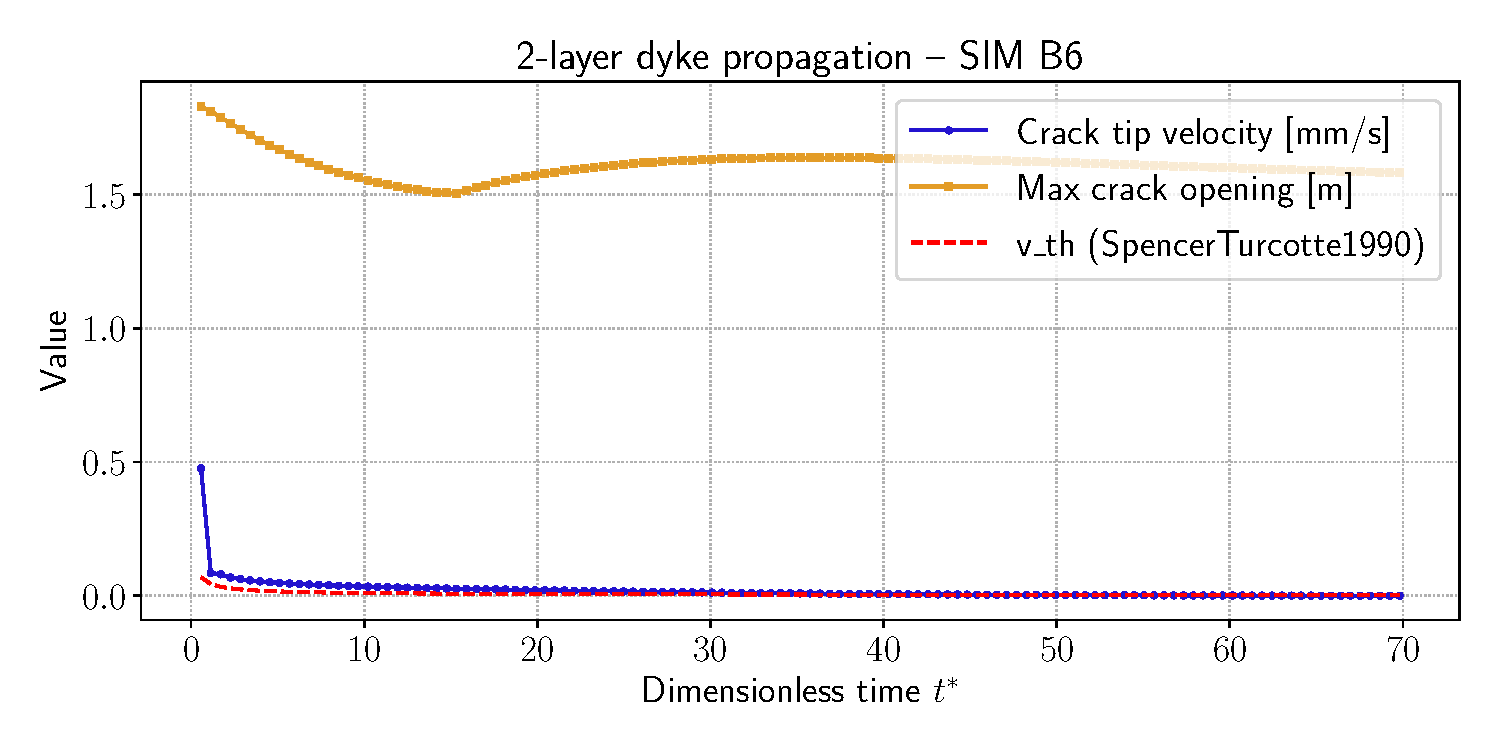
\includegraphics[width=0.5\linewidth]{/figs/fgs/2lay/case6/2l_veln_th_case6.pdf}
        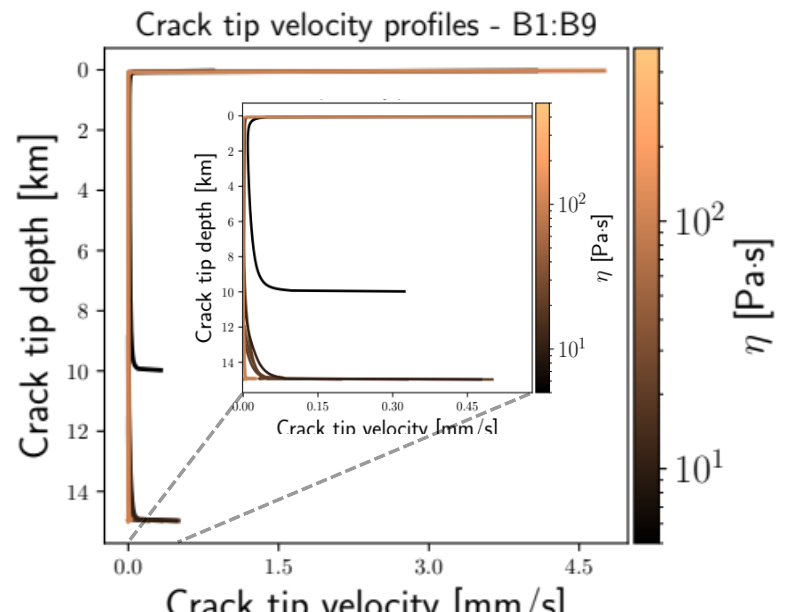
\includegraphics[width=0.5\linewidth]{/figs/fgs/2lay/zoom.png}
    \end{tabular}
  \caption{The accordance with the theoretical one, also seen in other runs not reported here (like B8, B3), could be due to a misleading search into different density variations values, since in order to maintain the iteration convergence, the viscosity was left unchecked. Nevertheless, the BE discretization is fine enough to capture tip fields in the $t^{\star} \gg 1$ regime, therefore asymptotic tip solutions seem to match pretty well in all simulations, as one should expect.}
\end{table}
\end{frame}

\begin{frame}{\textbf{Numerical velocity computation - case B2,B4,B3,B8}}
More cases are shown here:
\begin{table}
    \centering
    \begin{tabular}{cc}
        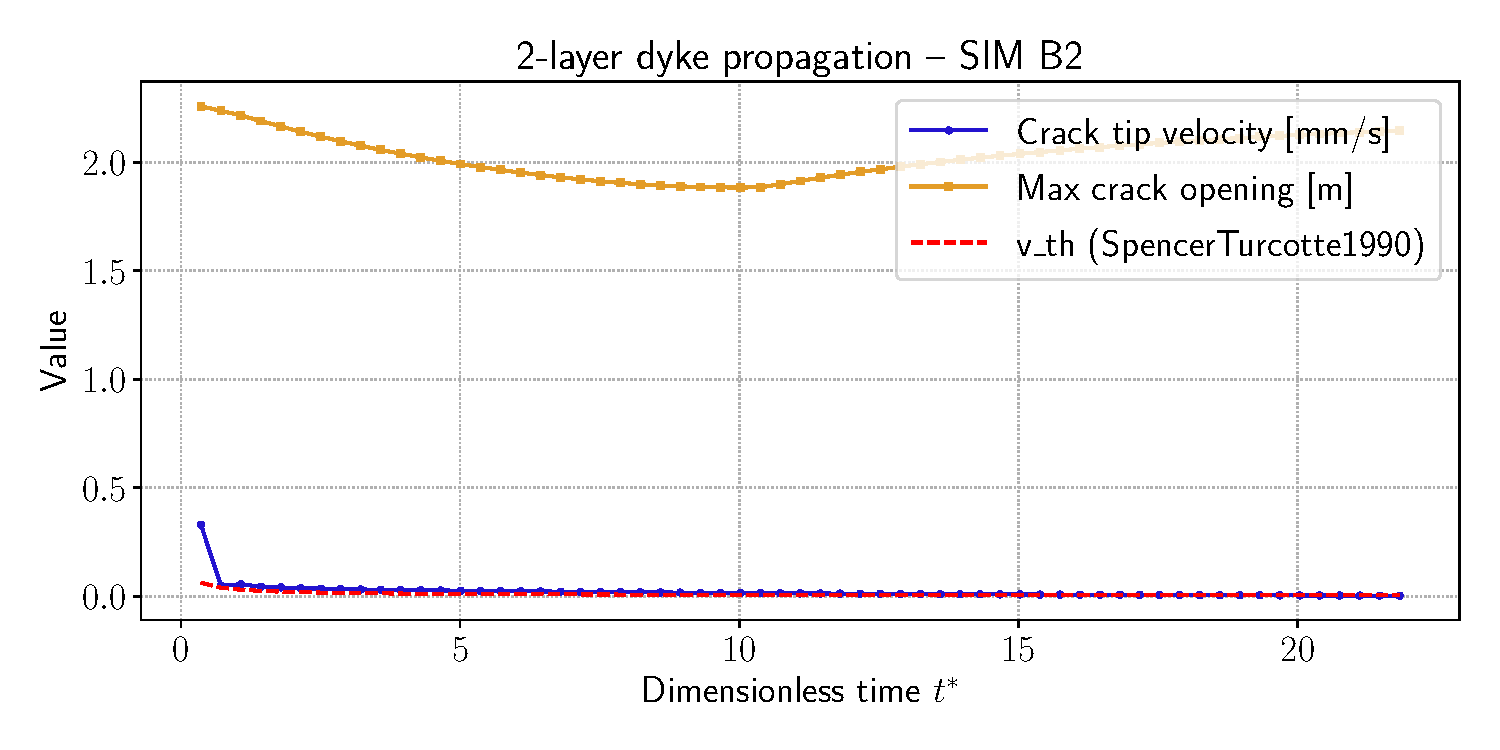
\includegraphics[width=0.5\linewidth]{/figs/fgs/2lay/case2/2l_veln_th_case2.pdf}
        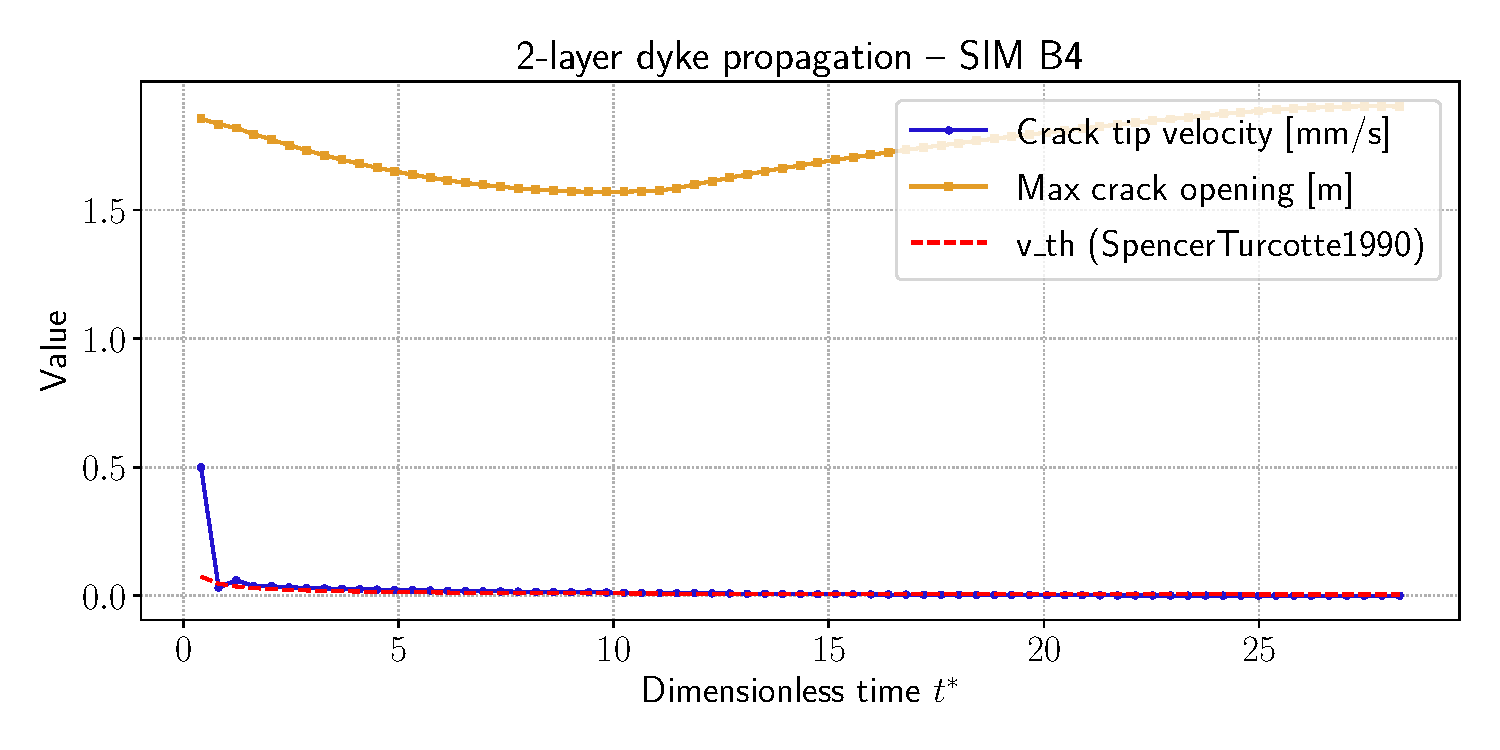
\includegraphics[width=0.5\linewidth]{/figs/fgs/2lay/case4/2l_veln_th_case4.pdf}\\
        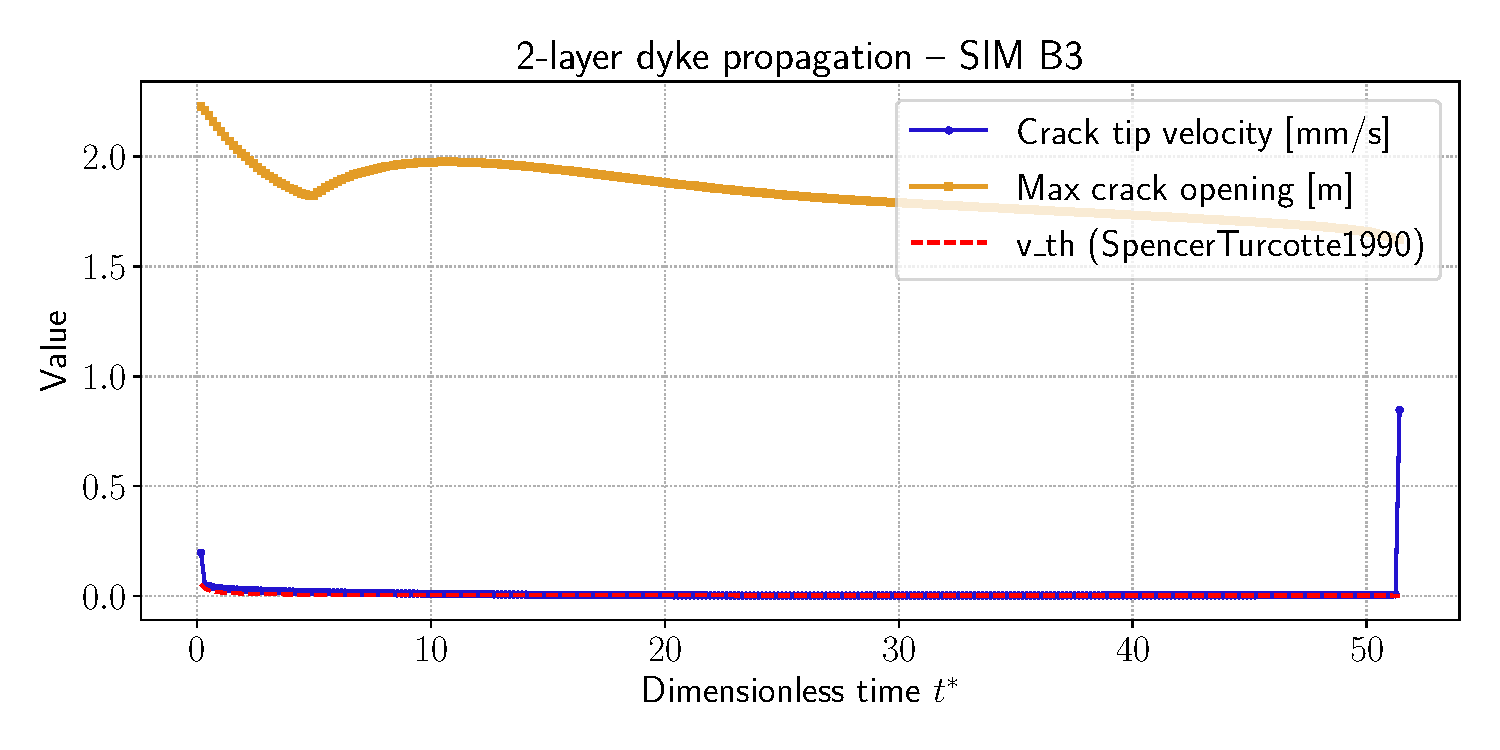
\includegraphics[width=0.5\linewidth]{/figs/fgs/2lay/case3/2l_veln_th_case3.pdf}
        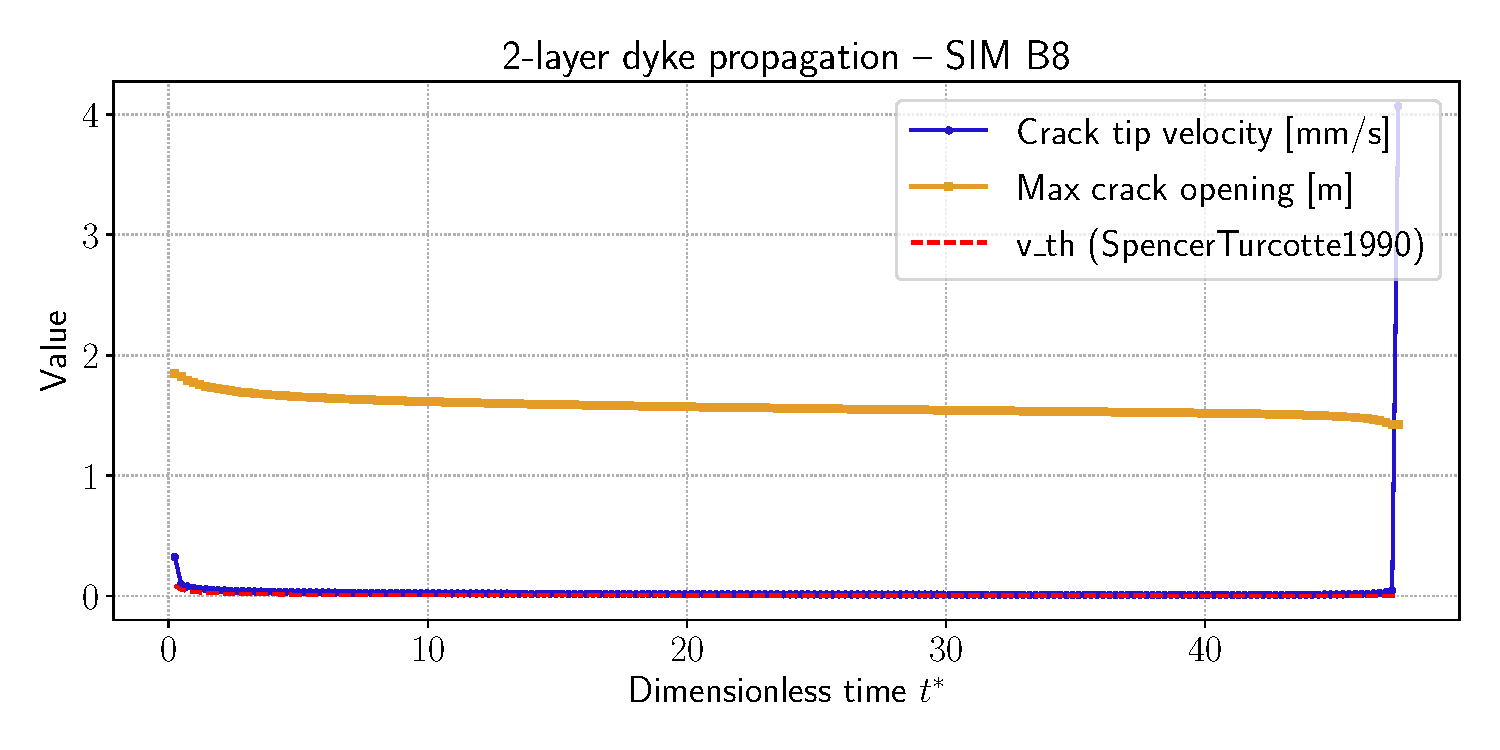
\includegraphics[width=0.5\linewidth]{/figs/fgs/2lay/case8/2l_veln_th_case8.pdf}
    \end{tabular}
\end{table}
\end{frame}


\begin{frame}{\textbf{Energy variation throughout the runs - case B3,B4,B5,B6,B1,B9}}
The Figure \ref{fig:5}, shows the energy trend for selected runs in the two-layer case.
\begin{columns}
% Column 1
\begin{column}{0.35\textwidth}
\Fontvi
A pronounced early peak suggests an initial fast-release phase (initial pressurization) followed by a another fast decline (B6), because viscous dissipation, due to its low value, can reduce the incremental energy per step. After transients (ex: B3,B9), $\Delta E$ keeps an approximately constant value, indicating steady propagation with balanced input and losses. The plateau seems independent of the value of the fracture toughness variation between the two layers though.
\end{column}
% Column 2    
\begin{column}{0.8\textwidth}
    \begin{figure}
    \centering
        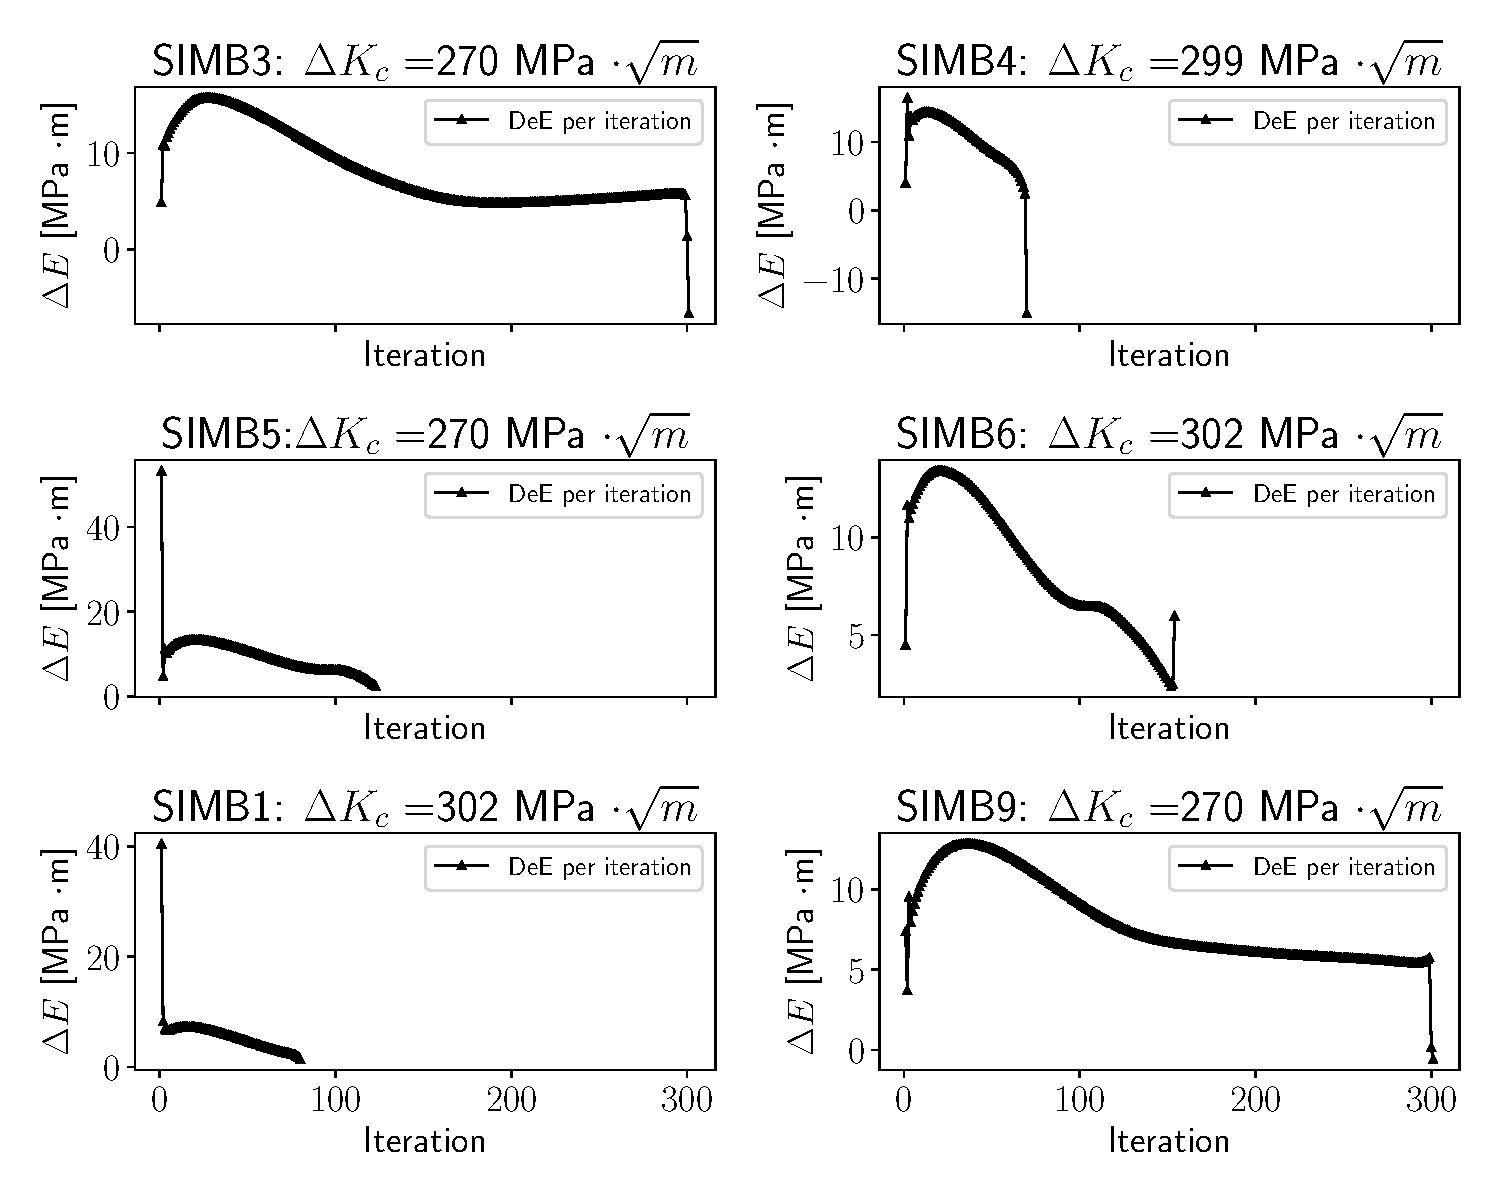
\includegraphics[height=0.7\linewidth]{/figs/fgs/2lay/2l_enrgvar.pdf}
            \label{fig:5}
    \end{figure}
\end{column}
\end{columns}
\end{frame}

\begin{frame}{\textbf{Velocity trend throughout the runs - case A1-8,B1-9}}
\Fontvi
The Figure \ref{fig:6}, shows the crack tip numerical velocities for selected runs in cases A-* while figure \ref{fig:7} shows the B-* ones. The iteration convergence is independent of the $v_i$ chosen after completing trial runs not shown here.
\begin{columns}
% Column 1
\begin{column}{0.6\textwidth}
    \begin{figure}
    \centering
        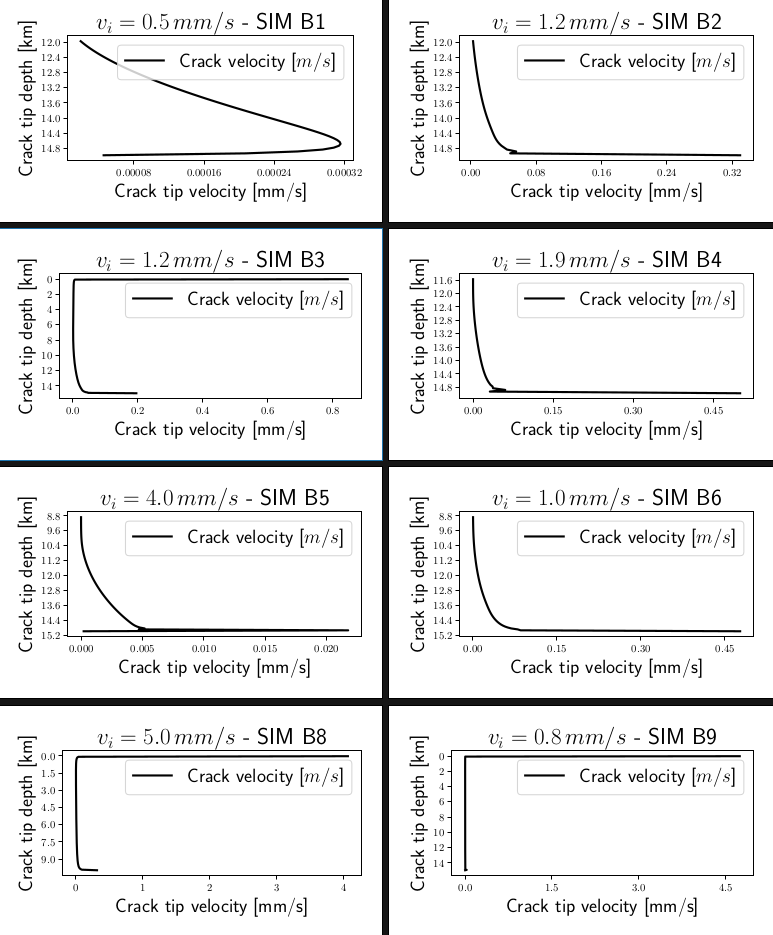
\includegraphics[height=0.98\linewidth]{/figs/fgs/collage/2l/vel_teo_case1-9.png}
            \label{fig:6}
    \end{figure}
\end{column}
% Column 2    
\begin{column}{0.6\textwidth}
    \begin{figure}
    \centering
        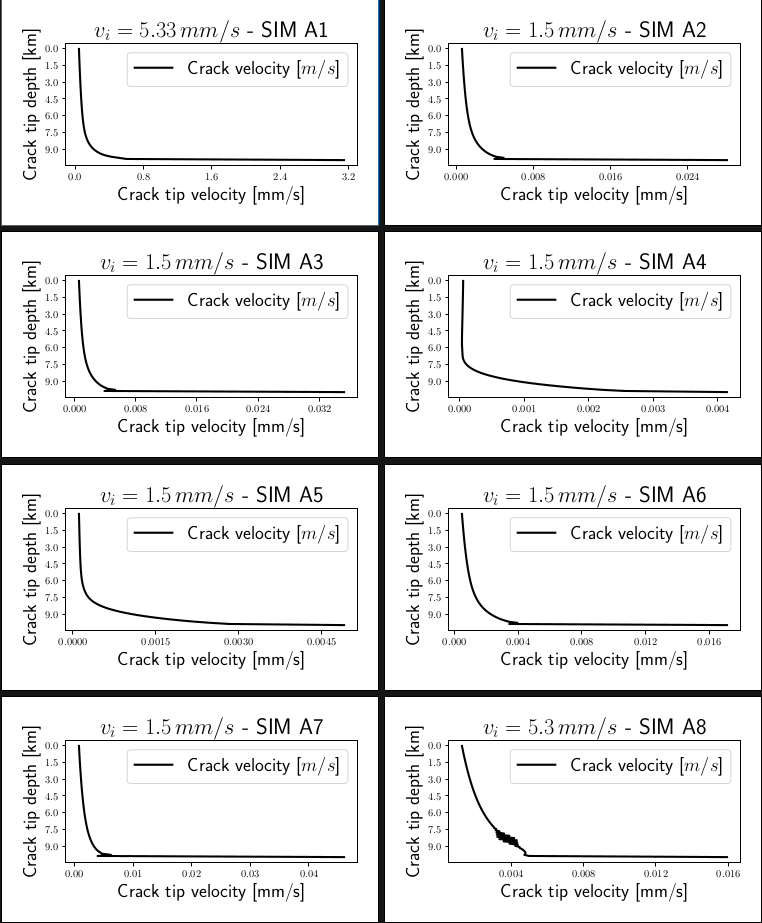
\includegraphics[height=0.98\linewidth]{/figs/fgs/collage/1l/veloc_depth.png}
            \label{fig:7}
    \end{figure}
\end{column}
\end{columns}
\end{frame}

\begin{frame}{\textbf{Crack shape and overlay in selected run - case B3}}
Below Figure \ref{fig:8}, show the geometry evolution for the case B3 with $\Delta \rho =100 \, dg/cm^3, \, \rho_f= 2.7 \, kg/dm^3, \, K_c=10\, GPa.$
\begin{table}
    \centering
    \begin{tabular}{cc}
        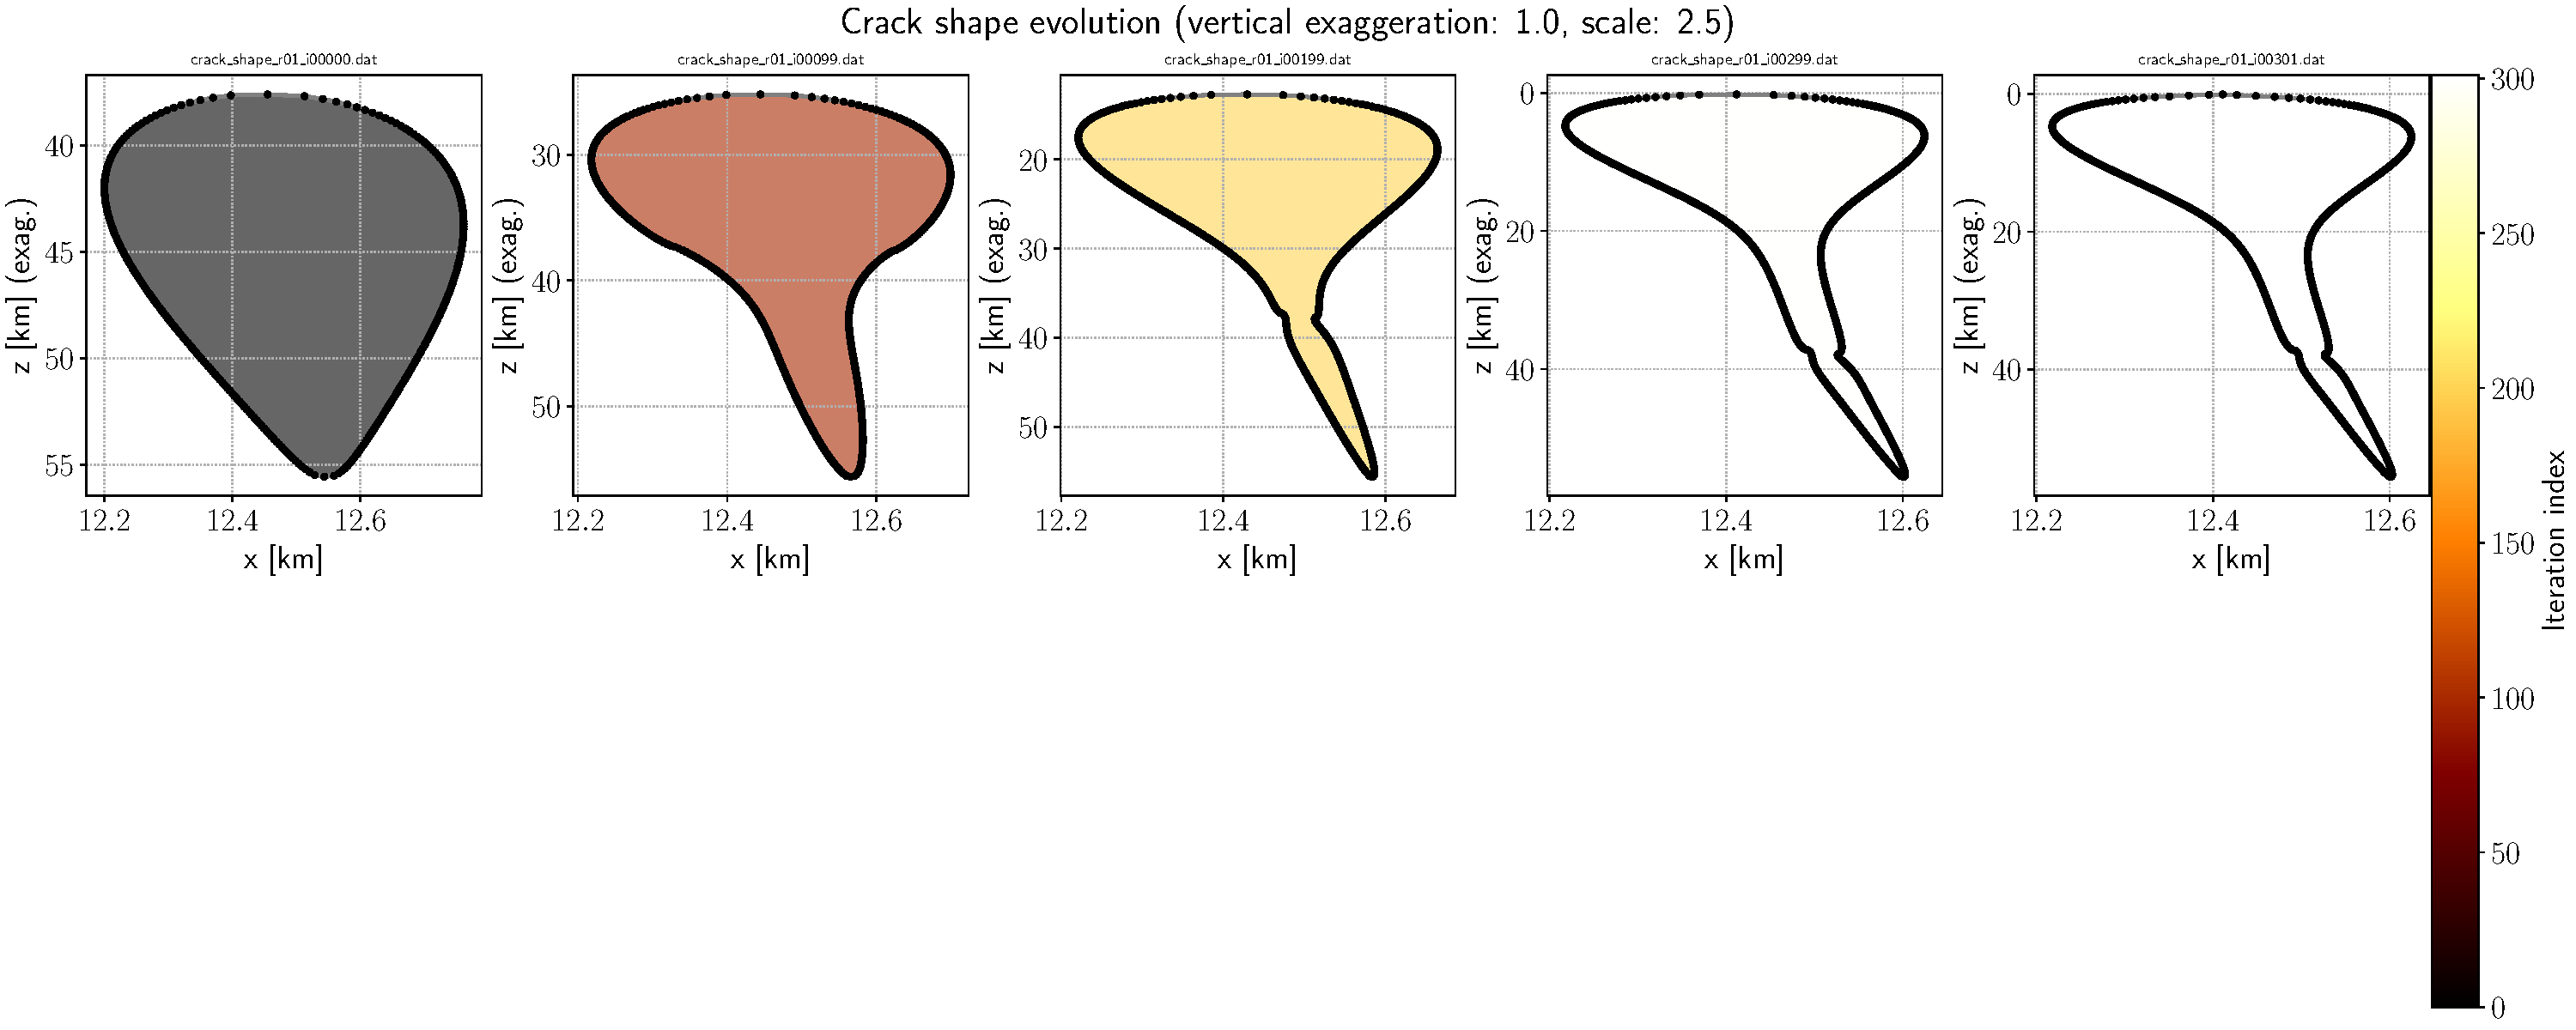
\includegraphics[width=1.0\linewidth]{/figs/fgs/2lay/case3/2l_crck_shp_case3.pdf}
    \end{tabular}
    \label{fig:8}
  \caption{In the two-layer simulations the dyke does not remain purely vertical; upon approaching the lithological interface it deflects laterally and develops a characteristic two-lobed morphology. This behavior is due to a mismatch in elastic properties across the interface that reduces the energy release rate for forward propagation, as well as a viscous redistribution of magma which implies a lateral deposit along a weaker interface. Increasing elastic contrast or reducing fracture toughness enhances lateral spreading. A more "blunted" tip is observed at higher viscosities, suggesting reduced stress intensity and slower fracture advance, as it was the case for the B9 case. }
\end{table}
\end{frame}

\begin{frame}{\textbf{Crack shape and overlay in selected run - case B8}}
Below Figure \ref{fig:9}, show geometry evolution for the case B8 with $\Delta \rho =300 \, dg/cm^3, \, \rho_f=\, 2.5 \, kg/dm^3, \, K_c=\, 19 GPa.$
\begin{table}
    \centering
    \begin{tabular}{cc}
        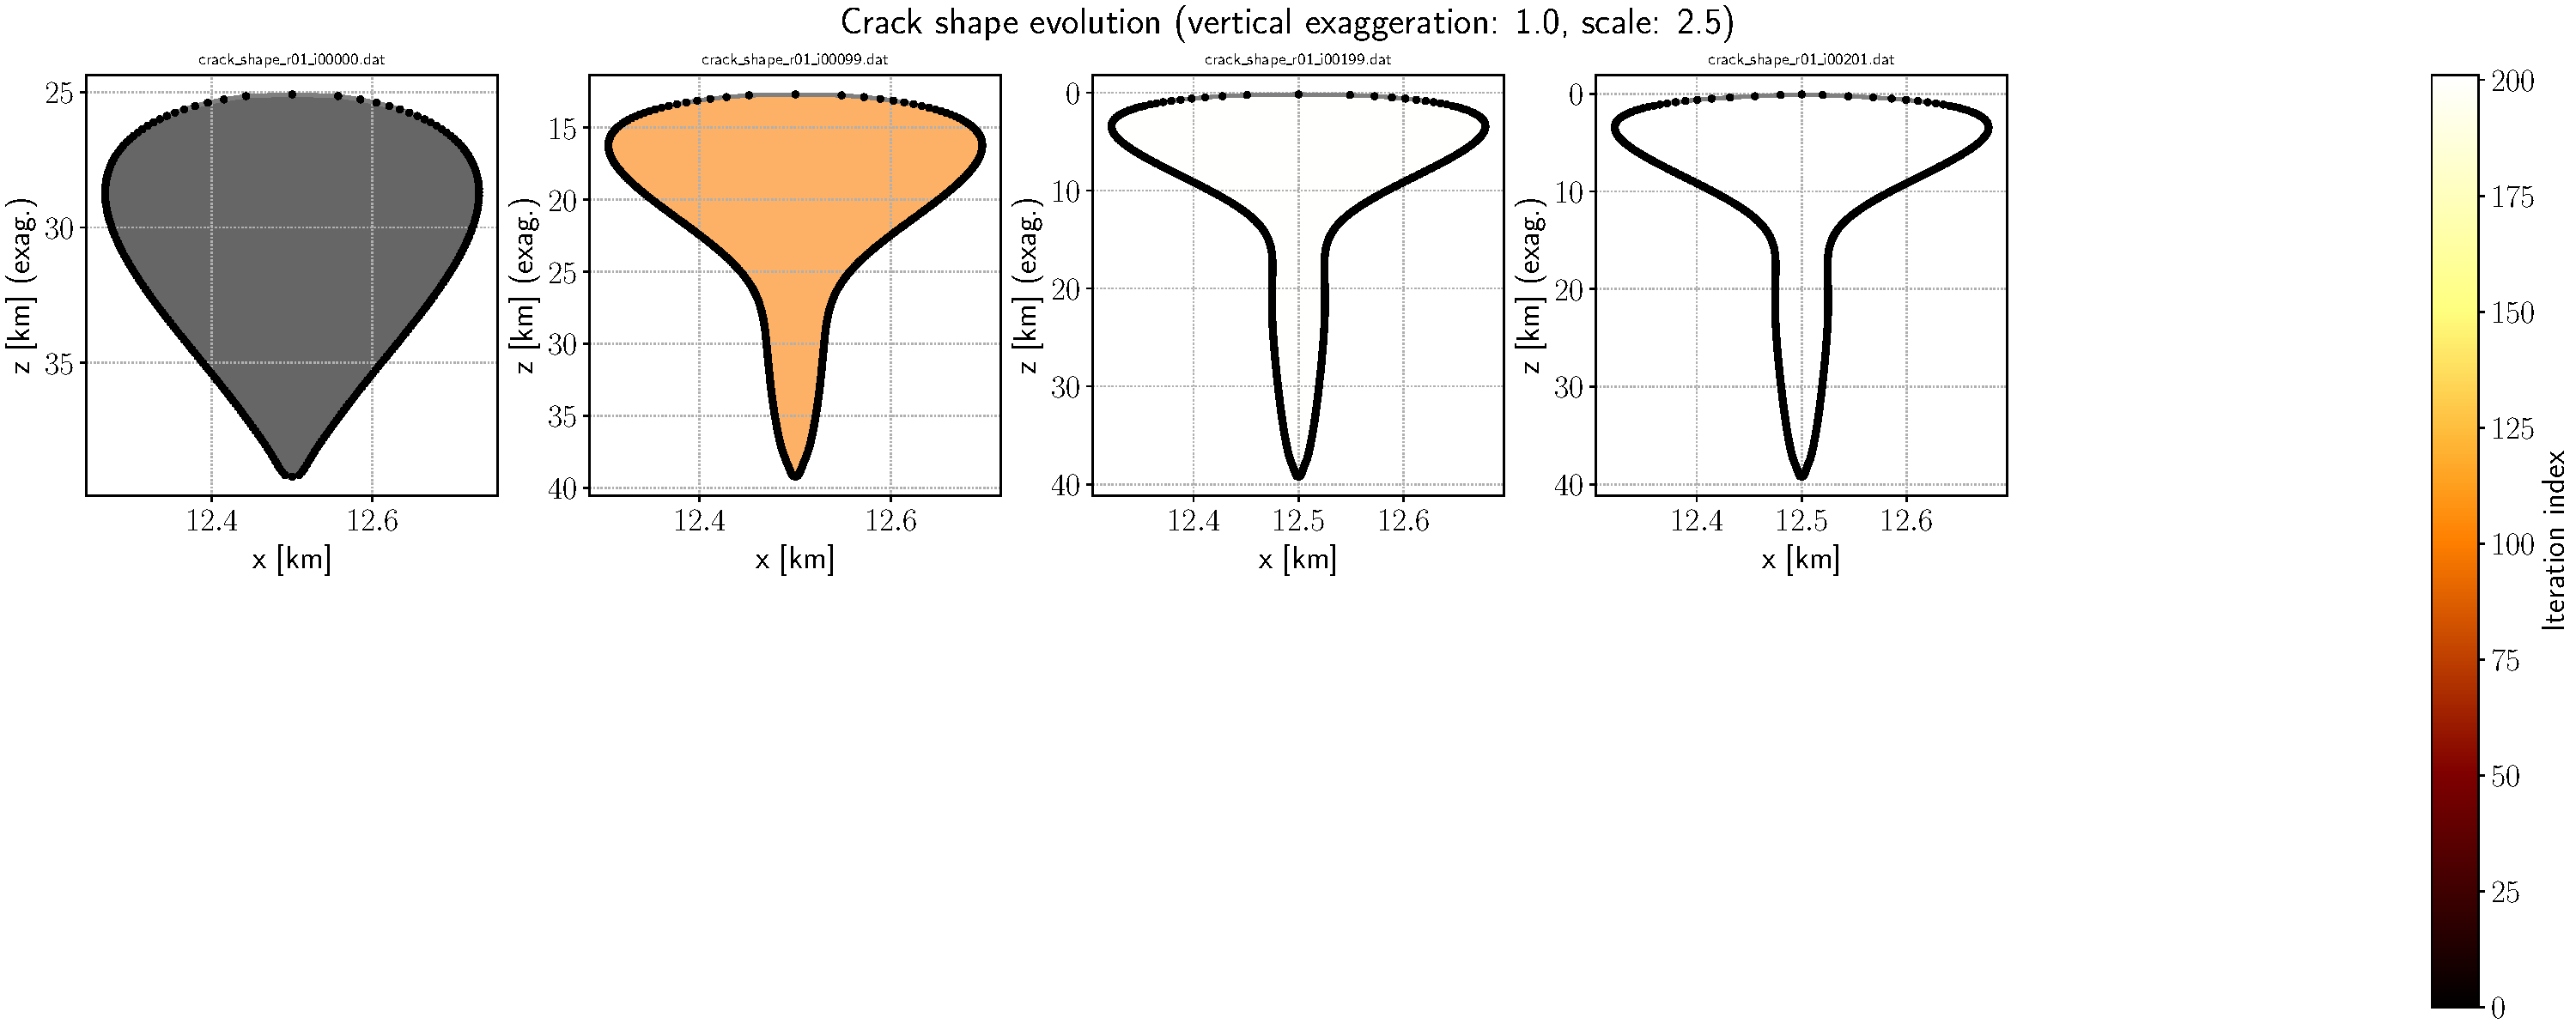
\includegraphics[width=1.05\linewidth]{/figs/fgs/2lay/case8/2l_crck_shp_case8.pdf}
    \end{tabular}
    \label{fig:9}
  \caption{If aperture and viscosity produce strong viscous resistance, flow can favor lateral paths of lower resistance producing lobes instead of forward propagation. Where driving pressure is sufficient to propagate, the crack opens; where resistance is higher it chooses lateral routes, creating lobes where opening is easier. This was the case since a compressional horizontal stress regime was applied to see the effects on the fluid filled fracture propagation.}
\end{table}
\end{frame}

\begin{frame}{\textbf{Crack shape and overlay in selected run - case B9}}
Below Figure \ref{fig:10}, show geometry evolution for the case B9 with $\Delta \rho = 0\, dg/cm^3, \, \rho_f=2.7 \, kg/dm^3, \, K_c=20 \, GPa.$
\begin{table}
    \centering
    \begin{tabular}{cc}
        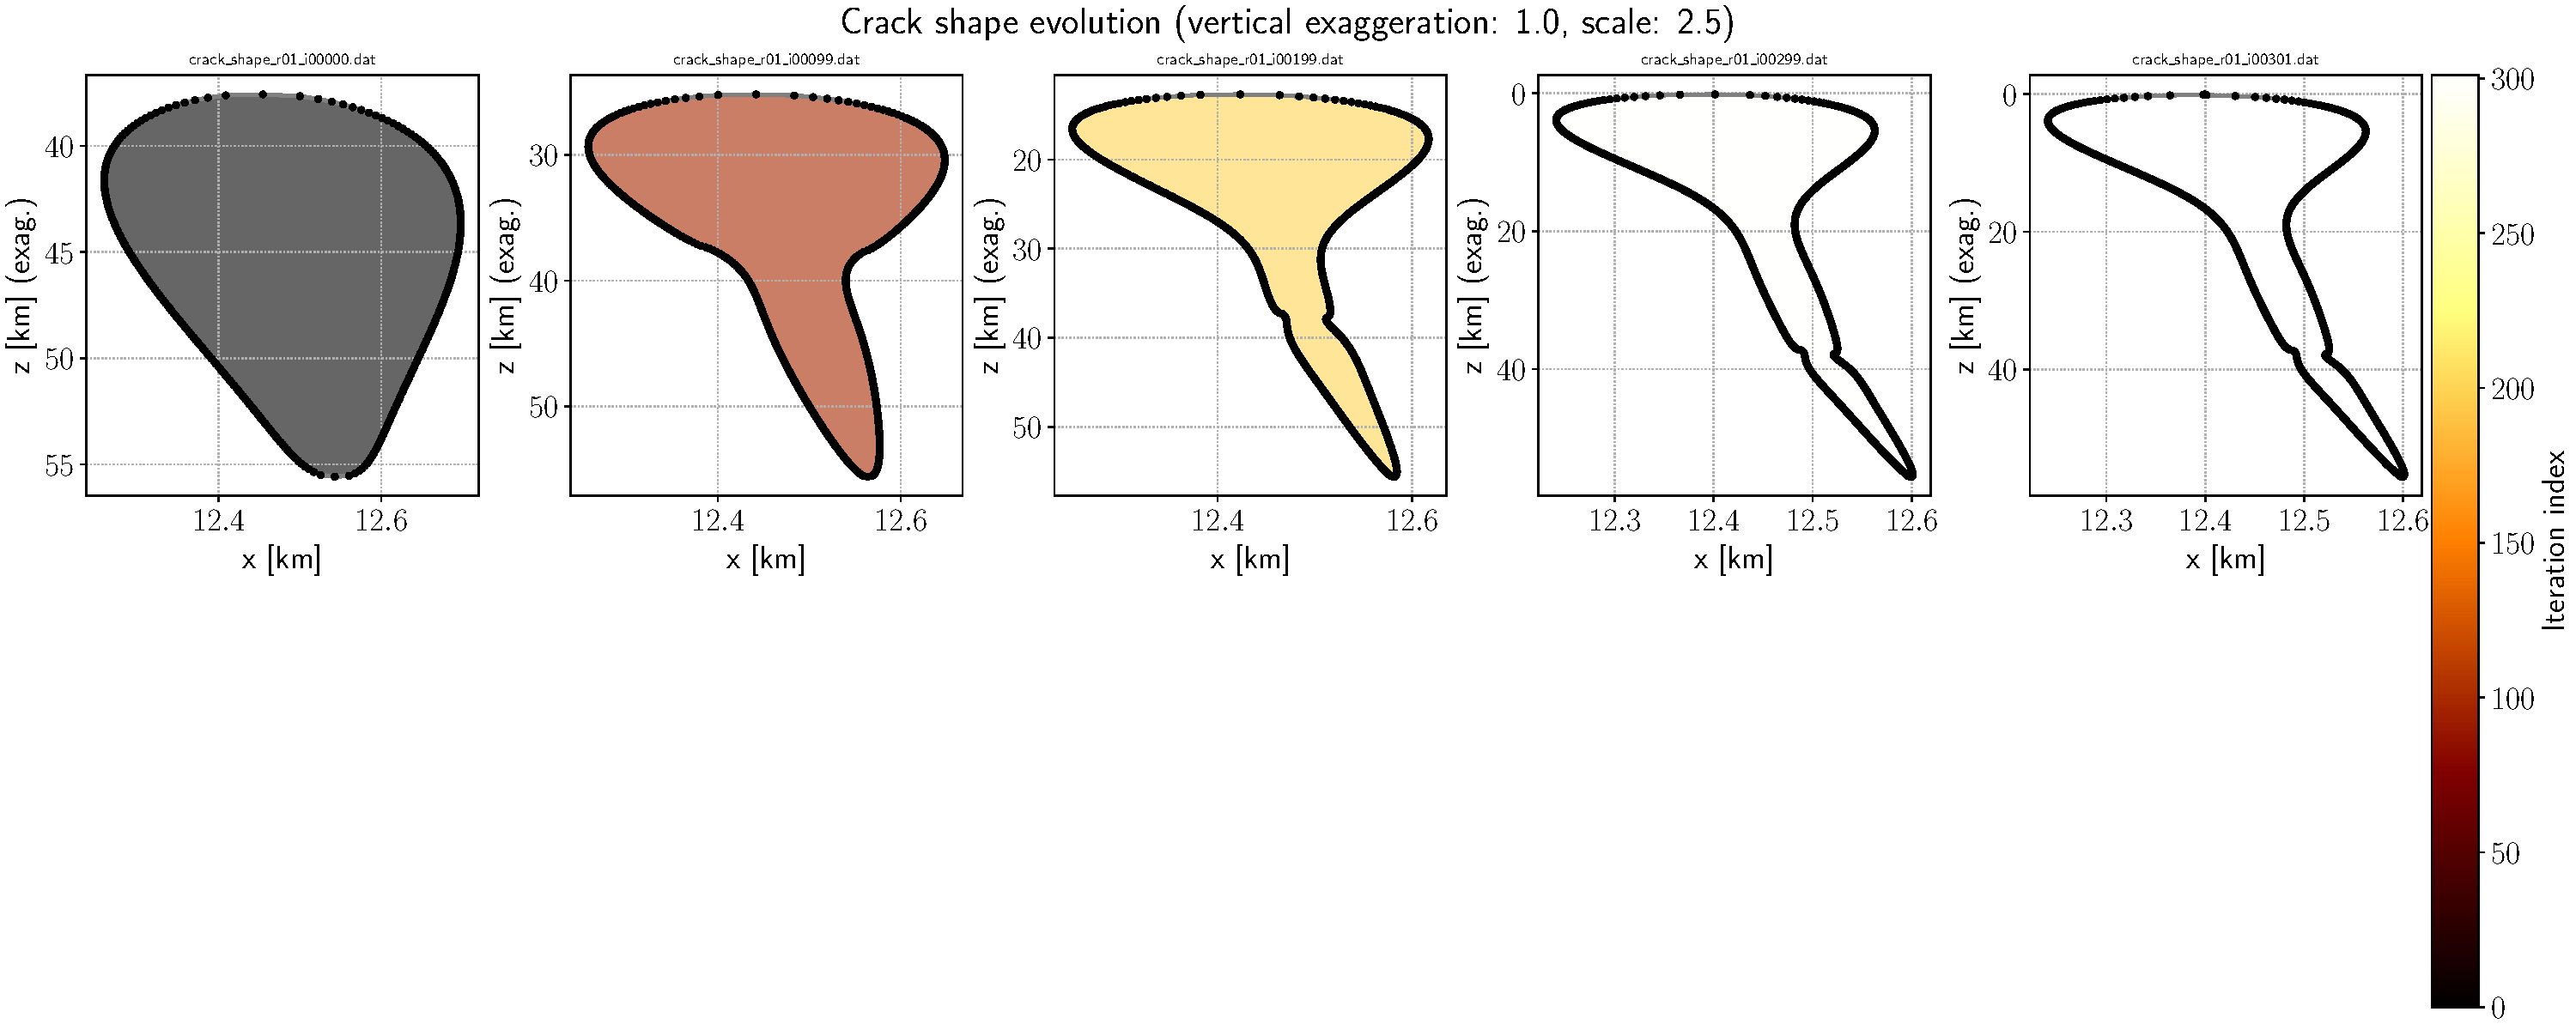
\includegraphics[width=1.05\linewidth]{/figs/fgs/2lay/case9/2l_crck_shp_case9.pdf}
    \end{tabular}
    \label{fig:10}
  \caption{The dyke reaches or approaches a layer interface where elastic contrast (stiffness/density) causes the crack to deflect laterally instead of continuing straight. The result is lateral spreading along the interface and lobes on either side of the tip. This cannot only be due the zero density contrast, which can induce a buoyancy change at the interface, but is likely due to the high value of both magma bulk modulus and viscosity, namely $100 Pa \cdot s$.}
\end{table}
\end{frame}


\begin{frame}[allowframebreaks]{\textbf{Conclusions and final remarks}}

\begin{enumerate}
\item \textbf{Dyke shape} In two-layer scenarios, the dyke commonly deflects laterally at layer interfaces, developing a two-lobed morphology. This is connected to elastic contrasts and high magma viscosity/bulk modulus, which promote lateral spreading over continuous vertical propagation.
\item \textbf{Velocity} Simulated crack tip velocities show good agreement with theoretical asymptotic solutions in the $t^{\star} \gg 1$ regime, confirming that the BE discretization resolves near-tip fields accurately.\\ Some matches may, however, be coincidental when viscosity was not adjusted alongside density contrasts to maintain convergence. A broader search into more parameters choice must be followed in the future. 
\item \textbf{Energy release} Sharp tip peaks indicate stress concentration and fracture toughness control, whereas mid-crack maxima suggest local stiffness variability. \\ Propagation arrest beyond certain iterations is consistent with insufficient tip driving pressure, especially at higher viscosities, where blunter tips and slower fracture advance are observed, namely the energy plateaus mentioned before.
\end{enumerate}
\end{frame}

\begin{frame}[allowframebreaks]{\textbf{Bibliography}}
\Fonttab
\scriptsize
\bibliographystyle{apalike}
\bibliography{bib/references}
\end{frame}
\end{document}
